\chapter{\textit{Resultados e Discussões}} \label{ch:resanddisc}

Neste Capítulo traremos os resultados obtidos nas aplicações das ORP e das ASA. Além disso, ao longo do texto, discutiremos alguns aspectos de suas implementações, bem como do resultados obtidos. Para esta tarefa, precisaremos ampliar mais nossa discussão acerca das turmas e dos processos de aplicação descritos no Capítulo \ref{ch:apl}. 

Separamos as Seções deste Capítulo de forma a analisarmos cada uma das três ORP e das três ASA de forma independente. As conexões entre as diferentes aplicações, bem como motivações que levaram ao processo de \textit{redesign} também serão descritas.

\section{Aplicações das ORP}

As Oficinas de Resolução de Problemas formam um conjunto de atividades didáticas estruturadas para testar a metodologia de \textit{Scaffolding} em turmas de Ensino Superior. No total foram realizadas três aplicações das ORP.

Essas aplicações possuem dois \textit{designs} distintos. Cada um deles adaptado para as especifidades de seus contextos de aplicação. Na Tabela \ref{tab:aplORP} podemos ver um resumo das informações básicas das turmas em que cada ORP foi realizada.

\begin{table}[ht]
\centering
\caption{Resumo das aplicações das ORP.}
\label{tab:aplORP}
\begin{adjustbox}{max width=\textwidth}
\begin{tabular}{lllllll}
\toprule
& \textbf{Forma} & \textbf{Curso} & \textbf{Semestre} & \textbf{Matriculados} & \textbf{Concluintes} & \textbf{Aprovados} \\
\midrule
\textbf{ORP1} & Remota & Engenharia Civil & Primeiro & 26 & 20 & 15 \\
\textbf{ORP2} & Presencial & Matemática & Oitavo & 3 & 2 & 2 \\
\textbf{ORP3} & Presencial & Física & Sétimo & 2 & 2 & 2 \\
\bottomrule
\end{tabular}
\end{adjustbox}
\caption*{Fonte: Construção do Autor.}
\end{table}


Na Seção \ref{sec:orp1}, abordaremos a ORP1, analisando seu processo desde a concepção até sua aplicação. Em seguida, procederemos a uma discussão sobre o alcance dos objetivos propostos e se conseguimos ou não responder satisfatoriamente a eles. O mesmo procedimento será adotado nas Seções \ref{sec:2orp} e \ref{sec:3orp} para as ORP2 e ORP3, respectivamente. 

\subsection{ORP1} \label{sec:orp1}

Estamos, neste momento, interessados em analisar o processo da ORP1 como um todo, não apenas os critérios de sua formulação (descritos no Capítulo \ref{ch:apl}). Dessa forma, vamos focar mais no processo de aplicação do que nos dados. Com isso devemos ser capazes de analisar o todo, e não apenas os resultados.

Nosso público-alvo, como já havia sido mencionado, são alunos do Ensino Superior. Durante nossa primeira Oficina de Resolução de Problemas conseguimos desenvolver o trabalho em uma turma de Engenharia Civil. A turma foi escolhida por uma questão de facilidade de acesso. Pois o professor regente da turma era o orientador desta dissertação. Assim, o autor deste trabalho conseguiria participar da aplicação, no papel de tutor, sem problemas.

Esta oficina foi realizada na disciplina de Física Geral e Experimental I, que pertencia ao primeiro semestre do referido curso. Por se tratar de um conteúdo inicial de física do primeiro semestre do curso, o professor adotou o livro-texto “Fundamentos de Física”, volume 1, \citeonline{Halliday2009}.

A UFSM possui um sistema de biblioteca online, no qual os alunos tem aceso a diversos títulos de livros didáticos, e esta biblioteca possui uma versão atualizada do livro adotado. Foi importante essa escolha pois, lembrando, estávamos em período de isolamento social, e a maior parte dos alunos não tinha acesso aos livros impressos.

Além disso, o livro possui um sistema de classificação de dificuldade das questões que facilitam a escolha de quais problemas utilizar. Reconhecemos a dificuldade das questões, neste sistema, pela representação na forma de círculos. Cada problema tem representado ao lado entre 1 e 3 círculos. 

Quanto mais círculos, em teoria, mais difícil é a questão. A Tabela \ref{tab:halliday_dificuldade} resume os graus de dificuldade das questões encontradas em \citeonline{Halliday2009}. Vale aqui ressaltar que essa classificação das questões é válida para todos os volumes, não apenas o primeiro - incluindo \citeonline{Halliday2009vol2,halliday}.

Neste sistema, se a questão é caracterizada com um círculo apenas, entendemos que seu processo de resolução passe pela aplicação direta de uma equação. Dessa forma, de acordo com \citeonline{Echeverria1998}, podemos classificar esta questão como sendo um exercício, e não um problema.

As questões marcadas com dois círculos necessitam de um entendimento maior acerca do conteúdo. Dessa forma, seguindo a classificação de \citeonline{Echeverria1998}, podemos definir estas questões como problemas.

Também podemos definir como problemas as questões marcadas com três círculos. Porém, neste caso, o processo de solução dos problemas passa pela necessidade de um aprofundamento maior no conteúdo, além de uma maior capacidade de raciocínio durante o processo de resolução.

Por causa da maior complexidade das questões com três círculos, optamos por não utilizá-las. Deveríamos dar prioridade às questões com dois círculos – que classificamos como problemas -, uma vez que as de um círculo correspondiam a exercícios. 

\begin{table}[ht]
\centering
\caption{Graus de Dificuldade das Questões de \citeonline{Halliday2009} e \citeonline{TiplerMosca2006}.}
\label{tab:halliday_dificuldade}
\begin{tabular}{@{}lcc@{}}
\toprule
\textbf{Tipo de Questão} & \textbf{Descrição} & \textbf{Grau de Dificuldade} \\
\midrule
\multirow{2}{*}{Fácil} & Conceitos básicos. & $\bullet$ \\
& aplicação direta de fórmulas. & \\
\midrule
\multirow{2}{*}{Médio} & Questões um pouco mais elaboradas. & $\bullet\bullet$ \\
& Requerem raciocínio lógico. & \\
\midrule
\multirow{2}{*}{Difícil} & Desafios complexos. & $\bullet\bullet\bullet$ \\
& Necessitam de análise cuidadosa. & \\
\bottomrule
\end{tabular}
\caption*{Fonte: Construção do Autor.}
\end{table}

A única exceção pensada para a utilização de questões de um círculo foi no caso de os alunos estarem com muita dificuldade no processo de resolução. Assim estas atividades funcionariam como forma de observar se a dificuldade se encontra nos conceitos físicos ou na parte matemática. Apesar disso, não houve a necessidade de reduzirmos o nível das questões apresentadas.

Foram realizadas oito atividades Síncronas (Apêndice \ref{ch:orp1}) e oito atividades Substitutivas (Apêndice \ref{ch:orp1subs}). Cada atividade substitutiva correspondia a uma atividade realizada em aula.

Para que os alunos pudessem estudar em casa, o professor regente passava listas de questões para que eles resolvessem. Essas listas não influenciavam nas atividades Síncronas nem nas notas dos alunos. Mas serviam de parâmetro para que os alunos estudassem em casa.

Por causa do pouco tempo para tirar dúvidas em aula, o tutor se mantinha à disposição da turma. O tutor poderia ajudar, neste caso, em dúvidas referentes à aula ou as listas de questões que o professor regente passava para casa, mas nunca para as atividades Síncronas ou Substitutivas.

A turma era, originalmente, constituída por 26 estudantes. Porém, seis destes alunos não compareceram às aulas ou não resolveram nenhuma atividade. Dessa forma, a turma contou com 20 alunos ativos (trabalhando em aula).

A evasão de alunos foi observada ao longo do semestre, e acredita-se que isso possa estar relacionado, entre outros fatores, à falta de adaptação ao modelo de ensino à distância adotado pela instituição. Esse fenômeno não se limitou apenas a esta turma, mas foi constatado em várias outras instituições de ensino durante a pandemia, conforme indicado por \citeonline{Palhares2022} em sua pesquisa. 

Para avaliar os alunos, ficou definido que o tutor corrigiria as atividades Síncronas com um peso máximo de 100 pontos. Dessa forma, caso os alunos obtivessem nota inferior a 80 pontos, poderiam optar por realizar a atividade Substitutiva.

As atividades Síncronas eram realizadas em horário de aula. As questões utilizadas neste caso foram escolhidas pelo professor regente da turma. Eram, ao todo, três versões diferentes da mesma questão para que os alunos resolvessem.

Já as atividades Substitutivas eram escolhidas pelo tutor, e retiradas de \citeonline{Halliday2009}. A escolha dessas questões estava baseada na análise feita pelo tutor das dificuldades durante a RP dos alunos. A pontuação máxima que os alunos poderiam tirar, optando por fazer as atividades Substitutivas, era de 80 pontos.

Assim, a questão escolhida para integrar a atividade Substitutiva deveria envolver o mesmo conteúdo e mesmo processo de resolução da atividade Síncrona, mas ter um enfoque nas dificuldades apresentadas pelo grupo de alunos.

Uma das preocupações, tanto do professor regente quanto do tutor, era que os alunos não trabalhassem nas atividades e acabassem copiando as respostas. Por causa disso as atividades Síncronas tinham três versões com valores diferentes. Porém o mesmo procedimento não pode ser tomado nas atividades Substitutivas.

Por causa disso, ao corrigir as Substitutivas, o tutor permanecia atento às semelhanças e diferenças nas resoluções dos alunos. Dessa forma, o tutor percebeu que alguns padrões de respostas começaram a se repetir, já na atividade Substitutiva 4.

Percebeu-se, então, que alguns alunos pulavam etapas de resolução, faziam mudanças de unidades sem apresentar cálculos e até apresentavam de forma direta a resposta final, sem o devido desenvolvido. Ademais, alguns alunos começaram a apresentar resoluções completamente idênticas.

Ao investigar o que estava acontecendo, o tutor descobriu que as questões utilizadas nas atividades Substitutivas estavam resolvidas passo a passo na internet. Inclusive com vídeos mostrando os passos e explicando a resolução. Ao assistir alguns desses vídeos, o tutor constatou que as respostas dadas por alguns alunos eram idênticas às dos vídeos.

Para evitar que isso continuasse acontecendo, optamos por utilizar o livro "Física para Engenheiros e Cientistas", volume 1, de \citeonline{TiplerMosca2006}. Este material foi escolhido por três motivos: possui um sistema de classificação de questões similar ao mostrado na Tabela \ref{tab:halliday_dificuldade}; também faz parte da biblioteca digital da UFSM; é mais difícil encontrar suas resoluções \textit{online}.

Ao término do semestre letivo foi disponibilizado um questionário, disponível no Apêndice \ref{ch:questORP1}, ao qual os alunos poderiam responder de forma anônima. Infelizmente poucos alunos responderam ao questionário. Além disso, por questões de ordem técnica que estavam fora de nosso controle, o servidor que armazenava as respostas dos questionário deletou os arquivos de forma definitiva.

Ou seja, dos quatro instrumentos descritos na Seção \ref{subsec: primeiraof} somente teríamos três para fazer a análise dos resultados (anotações do tutor, folhas de resolução e notas dos alunos). Este se tornou um dos principais motivos que levaram à reaplicação da metodologia.

\begin{figure}[ht]
\begin{center}
\caption{Gráfico da frequência de atividades entregues na ORP1.}
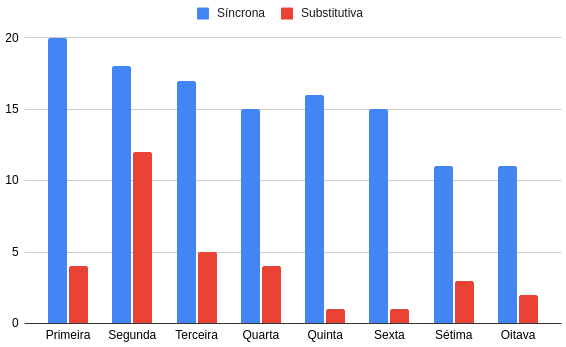
\includegraphics[width=0.7\textwidth]{fig/numerodeatividadesrealizadasORP1.png}
\label{fig:ativsORP1}
\caption*{Fonte: Construção do Autor.}
\end{center}
\end{figure}

A Figura \ref{fig:ativsORP1} que apresenta o gráfico da frequência de atividades entregues na ORP1. Em azul representamos o número de atividades Síncronas que foram entregues pelos alunos, e em vermelho o número de atividades Substitutivas.

Analisando a quantidade de atividades Síncronas entregues, percebemos que apenas na primeira atividade tivemos todos os 20 alunos resolvendo as questões. Vamos salientar aqui que mesmo os alunos que não conseguissem realizar as atividades Síncronas poderiam realizar a atividade Substitutiva.

Caso o aluno optasse por realizar apenas a atividade Substitutiva, ele não sofreria penalidades. A única consequência seria a ausência do \textit{feedback} do tutor para auxiliá-lo. Devido a essa condição, muitos alunos parecem ter escolhido fazer somente a atividade Substitutiva, mesmo que isso resultasse em uma nota máxima menor.

É importante ressaltar novamente que estávamos vivenciando um período de isolamento social, e, nesse contexto, a saúde mental dos estudantes era uma das nossas principais preocupações. Não tínhamos a intenção de impor a todos a realização das atividades Síncronas, uma vez que não tínhamos conhecimento do impacto que essa situação estava causando em cada um deles. O bem-estar dos alunos era prioridade, e compreendíamos que eles poderiam estar enfrentando desafios significativos devido às circunstâncias vigentes.

Entretanto, ao observarmos os dados da Figura \ref{fig:ativsORP1} vemos que, mesmo somando os números de atividades Síncronas e Substitutivas entregues na oitava aplicação, não somamos os 20 alunos que tínhamos no início. Alguns fatores colaboraram para essa diminuição do número de alunos ativos na disciplina.

Em primeiro lugar, é frequente ocorrerem desistências em disciplinas de Física. Muitos estudantes não estão familiarizados com as demandas e exigências do curso. Inclusive, alguns alunos sequer iniciaram o semestre devido à modalidade de ensino remoto adotada.

Em segundo lugar, o impacto da pandemia e do isolamento social afetou significativamente a todos. O tutor relata que alguns alunos expressaram dificuldades em se sentirem aptos a estudar ou realizar as atividades dentro dos prazos estabelecidos, devido a questões de cunho pessoal decorrentes da situação vivenciada.

Em terceiro lugar, alguns estudantes, ao constatarem que já haviam alcançado a nota necessária para aprovação, optaram por redirecionar seu foco para outras disciplinas. É importante ressaltar que, caso um aluno não realizasse uma atividade, sua pontuação correspondente seria atribuída como zero.

\begin{figure}[ht]
\begin{center}
\caption{Gráfico das médias das atividades respondidas da ORP1.}
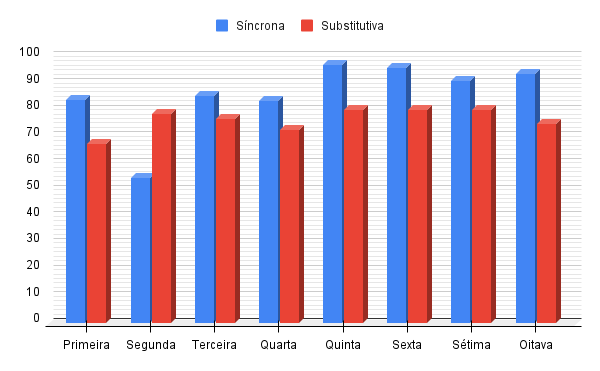
\includegraphics[width=1\textwidth]{fig/mediasORP1.png}
\label{fig:medORP1}
\caption*{Fonte: Construção do Autor.}
\end{center}
\end{figure}

Ao analisar a Figura \ref{fig:medORP1}, podemos obter uma visão geral das médias de cada uma das atividades realizadas pelos alunos. É importante ressaltar que, nesse gráfico específico, foram considerados apenas os valores das pontuações dos alunos que entregaram as atividades dentro do prazo estabelecido.

Com exceção da segunda atividade, em todos os outros casos, a média geral da turma foi maior nas atividades Síncronas. Essa diferença era esperada, visto que a pontuação máxima das atividades Síncronas é maior do que a das atividades Substitutas.

Entretanto, é importante notar que as atividades Substitutivas atingiram o platô em mais de uma ocasião. Isso significa que em diversos momentos, todos os alunos que optaram por realizar as atividades Substitutivas obtiveram nota máxima nessas atividades.

Na segunda atividade, é importante destacar que a média das atividades Substitutivas superou a das atividades Síncronas. Porém, é preciso ter um pouco mais de atenção a esse resultado, pois muitos alunos zeraram a atividade. No entanto, é notável que esses mesmos alunos apresentaram um progresso significativo ao longo da disciplina, obtendo notas cada vez maiores nas demais atividades.

\begin{figure}[ht]
\begin{center}
\caption{Notas finais ORP1.}
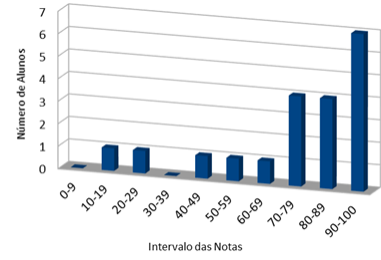
\includegraphics[width=0.8\textwidth]{fig/nfORP1.png}
\label{fig:nfORP1}
\caption*{Fonte: Construção do Autor.}
\end{center}
\end{figure}

Conforme observado nas Figuras \ref{fig:ativsORP1} e \ref{fig:medORP1}, ficou evidente que as atividades Substitutivas cumpriram seu papel de melhorar as notas dos alunos quando necessário. Embora a média geral das atividades Substitutivas seja menor do que a das atividades Síncronas, é importante ressaltar que a média individual dos alunos que optaram pela mudança sempre aumentou. Isso demonstra que as atividades Substitutivas foram efetivas em proporcionar uma oportunidade de melhoria para aqueles que precisavam.

A taxa de aprovação na disciplina foi de aproximadamente 60\%. No entanto, se considerarmos apenas os alunos que interagiram ao longo do semestre, o número sobe para 75\%.

Na Figura \ref{fig:nfORP1}, podemos observar o gráfico das notas finais dos alunos da ORP1. As notas estão divididas em intervalos, onde os alunos que foram aprovados foram aqueles que obtiveram nota igual ou superior a 70. Nota-se uma separação clara entre os alunos que atingiram essa pontuação mínima para aprovação e aqueles que não conseguiram.

A perda dos dados das respostas do questionário comprometeu nossos objetivos de pesquisa, especialmente no que diz respeito à compreensão das formas mais eficientes de dicas para os alunos (objetivo (d)). Devido a essa falta de informações, muitos questionamentos permaneceram vagos e sem respostas claras. A ausência dos dados prejudicou nossa capacidade de analisar de forma abrangente as percepções dos alunos e obter \textit{insights} significativos sobre o impacto do uso das dicas no processo de aprendizagem.

As notas dos alunos demonstraram uma melhora à medida que eles utilizaram o \textit{feedback} nas atividades Substitutivas quando necessário. Além disso, notamos uma redução no número de alunos precisando realizar as Substitutivas à medida que o semestre avançava, pois suas notas nas atividades Síncronas apresentavam um progresso contínuo. Essa correlação sugere que o uso do \textit{feedback} de forma apropriada pode ser um fator-chave para o aprimoramento do desempenho dos alunos e para sua maior eficácia nas atividades avaliativas em tempo real.

Por meio da análise das resoluções dos estudantes, constatou-se que aqueles que fizeram uso do \textit{feedback} durante as atividades Substitutivas exibiram um aprimoramento significativo no processo de RP. Alunos que inicialmente apresentavam dificuldades em extrair informações relevantes das questões, ao término do período letivo, demonstraram habilidade excepcional em resolvê-las com proficiência (objetivo \ref{item:c}).

Com base nisso, verificamos que os alunos adotavam uma abordagem semelhante à estratégia proposta por \citeonline{Pozo2009} ao resolver os problemas. Essa constatação limitou nossa capacidade de obter uma quantidade substancial de informações para a análise do objetivo específico \ref{item:a}.

Ao abordarmos o objetivo \ref{item:b} através das folhas de resposta, evidenciamos duas principais áreas que requerem suporte por parte dos alunos: aprofundamento na análise dos fenômenos físicos e reforço na aplicação prática dos conceitos matemáticos associados. Em muitos casos os alunos não sabiam interpretar a situação descrita pela questão, levando a resultados que não condizem com a realidade.

Além disso, ficamos surpresos com as dificuldades em matemática básica. Os principais erros encontrados envolveram o uso inadequado de operações matemáticas e a falta de habilidade na conversão de unidades. Não esperávamos encontrar tantas dificuldades nesse aspecto em uma turma de Ensino Superior.

Os dados coletados por todos os instrumentos revelaram uma diversidade significativa na turma em relação ao interesse pela RP ao longo do semestre. De fato, observou-se que os alunos demonstraram muito mais interesse em obter aprovação na disciplina do que em se engajar na resolução das atividades propostas.

É confirmado pelo tutor que o objetivo específico \ref{item:b} reflete as informações previamente verificadas pelas outras ferramentas. É nesse contexto que se destaca a maior necessidade de \textit{feedback}, que se concentra principalmente na parte matemática e na análise dos fenômenos descritos.

Entendemos que o objetivo \ref{item:d} não pôde ser totalmente respondido devido às semelhanças entre as dificuldades apresentadas pelos alunos, o que limitou a diversidade dos \textit{feedbacks} fornecidos. Entretanto, durante o processo de análise, surgiu a conscientização da necessidade de desenvolver uma classificação adequada para as dicas a serem utilizadas. Essa etapa é fundamental para garantir uma abordagem mais precisa e eficaz ao fornecer \textit{feedback} aos alunos, permitindo que eles recebam orientações específicas e relevantes para suas necessidades individuais.


\subsection{ORP2} \label{sec:2orp}

Após a conclusão da ORP1, dedicamos um período para estudar e analisar os resultados obtidos. Nesse ínterim, houve uma sinalização de que as aulas presenciais retornariam à UFSM. Diante dessa perspectiva, surgiu a necessidade de realizar um \textit{redesign} em nossa proposta, considerando essa mudança no cenário educacional. Esse processo de \textit{redesign} visa ajustar e adaptar nossa abordagem com base nas novas condições e possibilidades decorrentes do retorno das aulas presenciais, as quais podem impactar a dinâmica de ensino e aprendizagem.

Durante o período de estudos e análise, identificamos a possibilidade de haver diferenças no estilo e padrão de RP entre alunos principiantes e especialistas. Diante dessa constatação, nosso novo \textit{design} foi concebido para abordar duas turmas distintas.

A ORP2 foi aplicada à turma de principiantes, composta por alunos do curso de Licenciatura em Matemática - Noturno, na disciplina de Física II. Apesar de ser o oitavo semestre do currículo, esses alunos foram considerados iniciantes na RP de Física, uma vez que essa era apenas a segunda disciplina deles nessa área específica.

 A escolha da turma de principiantes para a ORP2 ocorreu pelos mesmos motivos da turma da ORP1, ou seja, devido ao fato do professor regente da disciplina também ser o orientador desta dissertação. Essa escolha facilitou a aquisição de informações e dados em um contexto geral da disciplina, permitindo uma abordagem mais detalhada e abrangente sobre a RP de Física nessa turma específica.

A Tabela \ref{tab:aplORP} revela que tivemos um número reduzido de apenas 3 alunos matriculados na turma. Apesar de não termos conhecimento antecipado desse baixo número de alunos, decidimos manter nossa forma de atuação conforme previamente estruturada na Seção \ref{sec:orp2e3}. Essa decisão foi tomada visando oferecer a melhor experiência possível aos alunos, garantindo que aqueles que se matricularam na disciplina recebessem o suporte e o acompanhamento necessário para o seu aprendizado e progresso acadêmico.

Durante as intervenções, o autor desta dissertação assumiu o papel de tutor da turma, responsável por auxiliar os alunos em suas dúvidas e fornecer as dicas necessárias para que alcançassem o progresso esperado nas questões. Como tutor, sua função era estar disponível para orientar os estudantes em seus estudos, esclarecer conceitos e oferecer suporte durante todo o processo de aprendizagem. Além disso, o tutor tinha a tarefa de fornecer as dicas apropriadas para ajudar os alunos a resolverem os desafios propostos, visando aprimorar seu desempenho nas atividades propostas. 

O livro utilizado como material didático na disciplina foi o "Fundamentos de Física", volume 2, de \citeonline{Halliday2009vol2}. A escolha desse livro foi motivada pelo fácil acesso dos estudantes, uma vez que o livro fazia parte da biblioteca virtual da instituição. Embora o ensino estivesse sendo retomado de forma presencial, a disponibilidade do livro digital facilitava o acesso dos alunos ao conteúdo, uma vez que a demanda pelos exemplares impressos era alta e poderia dificultar a retirada nas dependências da biblioteca.

Além disso, a escolha deste livro foi motivada pelo fato de ele utilizar o mesmo sistema de classificação de dificuldade das questões descrito na Tabela \ref{tab:halliday_dificuldade}. Isso possibilitou ao tutor montar as listas de questões, garantindo que nelas constassem apenas problemas, e não exercícios. Essa abordagem permitiu um maior enfoque em desafios conceituais e práticos, promovendo o desenvolvimento das habilidades dos estudantes na resolução de problemas complexos e na compreensão dos fundamentos da Física.

Na aplicação, os alunos resolveram as listas de exercícios em aula, na presença do tutor, e não nos preocupamos com possíveis cópias de resolução. A turma não era grande, o que facilitou o acompanhamento individualizado e tornou o controle sobre as cópias mais viável. A abordagem colaborativa proporcionou uma interação mais próxima e efetiva entre os estudantes e o tutor.

Foram aplicadas cinco listas de questões, detalhadas no Apêndice \ref{apendice:asa2}. Durante o início do processo, enfrentamos a dificuldade de selecionar o número ideal de questões a serem incluídas em cada lista. 

A primeira lista foi elaborada com 11 questões, com o intuito de abordar ao menos um problema representativo de cada tópico do capítulo trabalhado. Essa abordagem foi planejada para garantir que os alunos tivessem a oportunidade de praticar diferentes habilidades e conceitos abordados na disciplina, proporcionando uma visão geral dos temas tratados.


Durante a aplicação da primeira lista, identificamos que o tempo necessário para os alunos resolverem as questões era excessivamente longo. Os estudantes levaram cerca de 5 aulas para concluir a tarefa, o que estava além do tempo ideal, que seria de no máximo 2 aulas.

Compreendemos que a dificuldade enfrentada pelos alunos na resolução da lista estava relacionada tanto à própria natureza da RP em Física, uma vez que se tratava de uma turma de iniciantes nesse tipo de abordagem, quanto à quantidade de questões presentes na lista.

Dado que a turma era formada por estudantes novos na prática da RP, era natural que enfrentassem desafios em sua execução. No entanto, ao identificar que o número de questões também contribuía para o tempo excessivo de resolução, tomamos a decisão de reduzir a quantidade de questões nas próximas listas.

Essa abordagem visava proporcionar aos alunos uma experiência mais focada e menos sobrecarregada, permitindo-lhes dedicar mais tempo e atenção a cada problema apresentado. Acreditamos que essa adaptação contribuirá para que os estudantes se envolvam mais profundamente com cada tarefa, alcançando maior compreensão dos conceitos e desenvolvimento das habilidades em RP de Física.

Para otimizarmos o tempo de resolução das listas, decidimos por reduzir o número de questões em cada lista para 4. Essa escolha foi baseada em proporcionar aos alunos uma abordagem mais eficiente e focada, permitindo que dedicassem maior atenção e aprofundamento em cada problema apresentado.

As questões foram selecionadas cuidadosamente pelo tutor, visando englobar os pontos mais relevantes dos capítulos trabalhados, abordando diferentes conceitos e estratégias de resolução. Dessa forma, buscamos oferecer uma variedade de desafios que não se repetissem, promovendo um aprendizado mais abrangente e diversificado para os estudantes.

A execução da primeira lista de questões evidenciou uma dificuldade significativa por parte dos alunos em estabelecer conexões entre seus conhecimentos matemáticos e a aplicação desses conceitos nas questões de Física propostas. Esse cenário revelou a importância de trabalhar de forma mais gradual e cuidadosa na transição entre a teoria matemática e sua aplicação na RP de Física.

Diante dessa percepção, decidimos fornecer aos alunos algumas questões mais simples, envolvendo um círculo, com o objetivo de auxiliá-los a se familiarizar e se acostumar com o processo de RP de Física. Essas questões serviram como uma ponte para conectar os conceitos matemáticos aprendidos anteriormente às situações práticas e reais propostas nas questões de Física.

Essa abordagem foi fundamental para criar uma base sólida e confiante nos alunos, permitindo que eles desenvolvessem gradualmente a capacidade de utilizar seus conhecimentos matemáticos de forma eficiente na RP de Física. Ao longo do semestre, esse enfoque gradual possibilitou um progresso significativo nos resultados dos alunos e melhorou sua compreensão e confiança na abordagem de questões mais complexas de Física.

Ao longo do semestre, foram aplicadas cinco listas de problemas, cada uma correspondente a um capítulo do livro adotado. Dos três alunos matriculados na disciplina, apenas um deles acabou reprovando. Essa reprovação ocorreu antes mesmo do término do semestre, pois o estudante enfrentou dificuldades para comparecer regularmente às aulas.

A situação do estudante em questão parece ter sido afetada por problemas de disponibilidade de horários, o que o levou a não conseguir acompanhar as aulas regularmente. Infelizmente, essa ausência constante acabou impactando negativamente seu desempenho acadêmico, resultando na reprovação na disciplina.

É importante ressaltar que as intervenções realizadas durante o semestre buscavam auxiliar os alunos no desenvolvimento das habilidades necessárias para a RP de Física e, ao mesmo tempo, levar em consideração as particularidades e dificuldades individuais de cada estudante. Apesar do resultado negativo de um dos alunos, é possível observar que houve uma taxa de aprovação foi de aproximadamente 67\% (2 de 3 alunos), considerando a reprovação mencionada anteriormente.

Compreendemos as limitações impostas pela pequena quantidade de alunos na turma, o que pode ter afetado a confiabilidade dos resultados obtidos e limitado a capacidade de resposta aos objetivos do trabalho. É importante reconhecer que a amostra reduzida pode impactar a generalização dos resultados e dificultar a obtenção de conclusões mais abrangentes.

A turma com poucos alunos pode ter sido uma surpresa e, como fora mencionado anteriormente, não houve conhecimento prévio desse fato. Essa característica da turma pode ter influenciado os resultados obtidos, uma vez que a variabilidade dos dados pode ser menor, tornando mais difícil identificar padrões significativos.

No entanto, é essencial considerar que a realização da pesquisa e a coleta de dados são etapas importantes para o avanço do conhecimento científico. Mesmo que os resultados não tenham atingido a confiabilidade desejada, o trabalho realizado pode servir como ponto de partida para futuras investigações e aprimoramentos no campo de estudo.


No próximo \textit{redesign}, é fundamental reconhecer e mencionar as limitações do estudo, principalmente o tamanho da amostra. Uma turma composta por poucos alunos pode impactar os resultados, limitando a generalização dos achados. Para obter uma compreensão mais abrangente do tema, é importante buscar formas de superar essas limitações.

\subsection{ORP3} \label{sec:3orp}

A ORP3 foi realizada de forma concomitante à ORP2, com ambas utilizando o mesmo processo de avaliação. Os alunos foram avaliados por meio de listas de exercícios que deveriam ser resolvidas durante as aulas. Além disso, o andamento da disciplina dependia diretamente da evolução dos alunos nas atividades propostas.

Esse formato de avaliação em sala de aula permitiu um acompanhamento mais próximo do progresso dos estudantes, possibilitando ao tutor identificar eventuais dificuldades e fornecer o suporte necessário para o aprendizado. A abordagem de resolução de listas durante as aulas pode ter contribuído para o engajamento dos alunos, já que as dúvidas puderam ser sanadas de imediato e os conceitos aplicados de forma prática.

Dessa forma, a metodologia utilizada nas Oficinas proporcionou uma interação mais dinâmica entre tutor e alunos, permitindo uma avaliação mais precisa do conhecimento adquirido e a adaptação das estratégias de ensino conforme a necessidade da turma. Essa abordagem pode ter favorecido o aprendizado e o engajamento dos alunos ao longo da disciplina.

Na ORP3, a disciplina abordada foi Mecânica Quântica I, ministrada no sétimo semestre do curso de Física. Nessa etapa do curso, consideramos os acadêmicos como especialistas na RP de Física, uma vez que estavam prestes a concluir a graduação em Física.

A escolha de Mecânica Quântica I como disciplina para a ORP3 também foi influenciada por questões de conveniência e praticidade. O fato de o orientador desta dissertação atuar novamente como professor regente da disciplina possibilitou um acesso mais fácil e direto às turmas, permitindo uma maior integração e colaboração entre o professor e o autor deste trabalho, que desempenhava o papel de tutor.

A proximidade entre o professor regente e o tutor pode ter proporcionado uma melhor coordenação e alinhamento das atividades da disciplina com os objetivos da pesquisa em RP de Física. A atuação conjunta desses dois papéis também pode ter facilitado a identificação e seleção das questões mais relevantes e desafiadoras para as listas, garantindo uma abordagem mais efetiva na promoção do desenvolvimento das habilidades de resolução de problemas dos estudantes.

Na aplicação da ORP3, assim como na ORP2, também nos deparamos com um baixo número de estudantes matriculados. Apesar disso, decidimos manter o padrão de aplicação previamente desenvolvido, visando realizar uma análise comparativa mais consistente entre as duas turmas.


Na disciplina de Mecânica Quântica I, mesmo sendo uma disciplina avançada na graduação de Física, foi preciso realizar uma revisão de alguns princípios de Física Moderna com os estudantes. Para esse propósito, optamos pelo livro "Fundamentos de Física", volume 4, de \citeonline{halliday}, pelas mesmas razões já mencionadas para as ORP1 e ORP2. Essa abordagem permitiu reforçar conceitos fundamentais e nivelar o conhecimento dos alunos, proporcionando uma base mais sólida para o aprofundamento nos conteúdos de Mecânica Quântica.

Portanto, a primeira lista de questões na disciplina de Mecânica Quântica I teve como foco a revisão dos princípios da Física Moderna (Apêndice \ref{ch:orp3l1}). Semelhante à ORP2, que ocorria concomitantemente, observamos a necessidade de reduzir o número de questões para otimizar o tempo de resolução e proporcionar aos alunos uma abordagem mais eficiente e aprofundada em cada problema proposto.

A primeira lista abrangia 10 problemas para serem resolvidos, e os alunos levaram aproximadamente 3 semanas para completá-la. Após discussões com o professor regente, concordamos em reduzir o número de questões nas próximas listas, limitando-as a, no máximo, 4 problemas. 

Ao contrário da ORP2, onde as listas foram fixadas em 4 questões, na ORP3 optamos por deixar esta margem para o tutor na escolha do número de questões. Essa decisão foi tomada devido à natureza das questões da disciplina, que requeriam mais tempo, conhecimento e concentração por parte dos alunos. Dessa forma, permitimos ao tutor ajustar o número de problemas de acordo com a complexidade e abrangência dos tópicos abordados em cada lista, proporcionando uma melhor adaptação às necessidades da turma.

Para prosseguir com o andamento da disciplina e abordar os conteúdos próprios da Mecânica Quântica, o professor regente optou por utilizar o livro "Física Quântica" de \citeonline{Gasiorowicz1979}. Essa escolha ocorreu por acreditarmos que os alunos estariam preparados para enfrentar um material tecnicamente mais robusto.


Com base nas dificuldades encontradas ao tentar resolver algumas questões com os alunos em sala de aula, o professor regente percebeu que eles apresentam muita dificuldade em aspectos matemáticos. Diante disso, a utilização do livro de \citeonline{Gasiorowicz1979} poderia acabar prejudicando o desenvolvimento dos alunos. É importante considerar que a abordagem de um material mais avançado requer uma base sólida em matemática, e é fundamental garantir que os estudantes estejam devidamente preparados para enfrentar os desafios da Mecânica Quântica.

Após uma cuidadosa análise do professor e do tutor, optamos por adotar o livro "Mecânica Quântica" de \citeonline{Griffiths2011} como material principal para a disciplina. Essa escolha foi motivada pelas dificuldades dos alunos em relação aos aspectos matemáticos encontrados ao tentar resolver algumas questões com eles em sala de aula.

O livro de \citeonline{Griffiths2011} oferece uma abordagem mais moderna e clara, além de contar com questões complementares que enriquecem o aprendizado. Acreditamos que essa nova opção nos permitiria traçar um processo de ensino e aprendizagem mais simples e eficiente, auxiliando os alunos a superarem suas dificuldades e progredirem de maneira mais consistente no estudo da Mecânica Quântica.

Após a adoção do novo material, que ocorreu na primeira metade do semestre, foram aplicadas mais duas listas de exercícios (Apêndices \ref{ch:orp3l2} e \ref{ch:orp3l3}). Diferentemente do que ocorreu na ORP2, onde os alunos conseguiam realizar as listas dentro de uma ou duas aulas, os estudantes na ORP3 continuaram precisando de mais tempo para resolver as questões.

Entendemos que os alunos tenham apresentado a necessidade de trabalhar e tenham muitas obrigações fora da sala de aula, o que pode impactar diretamente o tempo disponível para estudar e resolver as listas de exercícios. Essa é uma realidade comum em muitos ambientes acadêmicos, e é importante levar em consideração os diversos compromissos e responsabilidades que os estudantes enfrentam.

Os alunos faziam questionamentos pertinentes ao tutor, mostrando que eles estavam engajados e interessados em aprender, buscando compreender os conceitos de forma mais aprofundada. No entanto, é natural que a RP, especialmente em uma disciplina complexa como a Mecânica Quântica, demande tempo e dedicação.

Para auxiliar os alunos nesse processo e permitir a continuação das aulas teóricas, decidimos permitir que os alunos entregassem algumas listas de forma remota. No entanto, para evitar plágios e garantir a integridade do processo de resolução, o tutor precisaria verificar o progresso individual de cada aluno, assegurando que cada resposta fosse original e resultado do esforço individual. 

Ao final do semestre, o comprometimento e esforço dos estudantes foram recompensados com a aprovação. No entanto, assim como na ORP2, a quantidade limitada de dados disponíveis para análise nos impediu de realizar uma análise mais abrangente dos objetivos propostos. 

Podemos observar alguns pontos em comum entre as ORP2 e ORP3. Ambas as turmas apresentaram um número reduzido de alunos, o que impactou na aplicação da proposta inicial. No entanto, mesmo com esse cenário, foi possível notar a participação ativa dos estudantes durante as aulas, com questionamentos pertinentes e interesse nas atividades propostas (segundo a análise do tutor). É importante ressaltar que, devido à limitação de dados, é necessário cautela ao interpretar quaisquer resultados, pois a falta de uma amostra maior pode comprometer a representatividade dos achados. 

\section{Aplicações das ASA}


Diante das dificuldades enfrentadas nas ORP2 e ORP3, bem como os problemas técnicos na coleta de dados na ORP1, foi necessário repensar nossas estratégias para obter resultados mais expressivos e consistentes. Para isso, uma abordagem promissora foi o aumento do tamanho das turmas, visando coletar dados de um maior número de alunos e tornar as análises mais confiáveis e representativas.

Compreendendo as dificuldades e desafios enfrentados no primeiro semestre de retorno às aulas presenciais, em que o Ensino Superior ainda sofria com os reflexos da alta evasão decorrente da Pandemia \cite{Palhares2022}, decidimos repensar nosso público-alvo para obter resultados mais consistentes e significativos. Diante da incerteza quanto ao crescimento do número de estudantes nas turmas de Ensino Superior, optamos por direcionar nossas intervenções para o Ensino Médio, onde já possuíamos conhecimento do número mais elevado de alunos.

As intervenções realizadas no Ensino Médio foram denominadas de ASA e são detalhadas na Seção \ref{sec:asa}. Ao contrário das ORP, que tinham a duração de um semestre, as ASA foram planejadas para serem aplicadas em um trimestre, devido à divisão dos períodos letivos na instituição. Essa alteração no cronograma permitiu um enfoque mais concentrado nas atividades e uma maior agilidade na coleta de dados e análise dos resultados. 

As ASA foram aplicadas durante os meses de março, abril e maio de 2023. Cada turma participou de três atividades ao longo desse período, com um espaçamento médio de um mês entre cada atividade. Cada uma dessas atividades consistia em quatro modelos (variações) distintas, propostas para dificultar plágio entre as resoluções dos alunos.

A decisão de direcionar nossas intervenções para o Ensino Médio foi facilitada pelo fato de o autor desta dissertação ser o professor regente das turmas selecionadas. Assim, a pesquisa foi realizada em uma Escola Particular Confessional no interior do Estado do Rio Grande do Sul, contemplando três turmas correspondentes a cada ano do Ensino Médio.

Compreendemos que a troca para o público-alvo do Ensino Médio, e consequentemente a inclusão de alunos de diferentes anos, impediu a análise específica das diferenças no processo de RP entre estudantes principiantes e experientes. De fato, essa abordagem permitiria investigar se os alunos mais velhos (do terceiro ano) demonstrariam maior habilidade e destreza na resolução de problemas, em comparação aos alunos de anos anteriores.

No entanto, é importante considerar que as dificuldades apresentadas pelas turmas, mesmo aquelas com alunos mais velhos, podem ser influenciadas pelas experiências de aprendizagem prévias em ambientes remotos. A transição para o ensino remoto durante o período de pandemia parece ter gerado desafios adicionais para os estudantes, como o acesso limitado aos recursos educacionais, a falta de interação presencial com os colegas e professores, e a adaptação a novas plataformas e metodologias de ensino \cite{Santos_Bastos_Souza_Figueiredo_Teixeira_Quintiliano_2021}.

\begin{table}[ht]
\centering
\caption{Informações básicas das turmas de aplicação das ASA.}
\label{tab:basicoASA}
\begin{tabular}{p{5cm}rrr}
\toprule
& \textbf{ASA1} & \textbf{ASA2} & \textbf{ASA3} \\
\midrule
\textbf{Alunos na Turma} & 24 & 26 & 19 \\
\textbf{Alunos Avaliados} & 16 & 21 & 14 \\
\textbf{Média de Idade (anos)} & 15 & 16 & 17 \\
\bottomrule
\end{tabular}
\caption*{Fonte: Construção do Autor.}
\end{table}

A Tabela \ref{tab:basicoASA} apresenta informações fundamentais sobre as turmas nas quais aplicamos as ASA. Nela, podemos observar que há variações na quantidade de alunos matriculados em cada turma, bem como nos alunos que efetivamente participaram das avaliações durante a aplicação das atividades. 

Entendemos que a discrepância na quantidade de alunos nas turmas que participaram das ASA pode ser atribuída a diferentes fatores. Dois dos principais motivos são o critério de considerar apenas os alunos que realizaram todas as atividades junto com a turma, bem como a presença de estudantes com laudos médicos que requerem acompanhamento e avaliações especiais. Essa abordagem visa manter a consistência na análise dos resultados, uma vez que a participação regular nas atividades é fundamental para avaliar o impacto das ASA na aprendizagem dos alunos.

Nas Seções \ref{subsec:asa1}, \ref{subsec:asa2} e \ref{subsec:asa3}, realizaremos uma análise individual das aplicações das ASA em cada uma das turmas do Ensino Médio. Ao final de cada seção, faremos uma conexão entre os dados obtidos nessas aplicações e os objetivos do trabalho proposto.

Adicionalmente, considerando que o professor regente (autor desta dissertação) já havia lecionado para as turmas anteriormente, é relevante fornecer um breve histórico sobre cada uma delas. Essa abordagem inédita no presente trabalho foi considerada benéfica, pois possibilitou utilizar essas informações na formulação do \textit{design} atual da pesquisa.

\subsection{ASA1} \label{subsec:asa1}

A ASA1 foi aplicada em uma turma de 1º ano do Ensino Médio. Conforme apresentado na Tabela \ref{tab:basicoASA}, a turma possuía um total de 24 alunos, mas para fins desta pesquisa, foram considerados apenas 16 deles. A escolha de excluir alguns alunos da análise se deveu a critérios específicos, como a participação em todas as atividades propostas e a presença de laudos médicos\footnote{Existiam alunos que eram diagnosticados com transtornos e dificuldades de aprendizagem, o que exigia uma avaliação adaptada para os mesmos. Estes alunos foram avaliados mas não foram considerados no estudo, pois suas atividades diferiam do restante dos estudantes analisados.} que pudessem interferir na proposta do estudo. 

O tutor já havia lecionado Matemática para esta turma no ano anterior, quando eles estavam no 9º ano do Ensino Fundamental II. Durante a transição para o Ensino Médio, a turma sofreu com a saída de muitos alunos, e os novos estudantes que ingressaram não compensaram essas perdas, resultando em um número menor de alunos na turma.

Durante o período de transição, alguns alunos ingressaram na turma apresentando laudos médicos e condições especiais, o que não era comum anteriormente. Esses estudantes acabaram por gerar desafios adicionais, pois suas necessidades requeriam um acompanhamento diferenciado e, em algumas situações, tumultuavam o ambiente durante as aulas.

A turma do 9º ano já apresentava desafios significativos em termos de disciplina e dificuldades de aprendizagem. Com a chegada dos novos alunos no Ensino Médio, essas questões foram agravadas, tornando o trabalho com a turma ainda mais desafiador. O ambiente de sala de aula se mostrou complexo devido à presença mais frequente de comportamentos disruptivos.

É importante ressaltar que esses estudantes enfrentaram condições de ensino adversas durante a Pandemia. No 7º ano, as aulas foram realizadas de forma remota, e no 8º ano, em formato híbrido. Essa transição entre modalidades de ensino pode ter afetado o engajamento e o desempenho dos alunos. Além disso, no 9º ano, houve uma flexibilização em relação às faltas na escola, considerando as dificuldades de adaptação dos estudantes durante esse período desafiador. Esses fatores podem ter contribuído para a dinâmica complexa da turma no Ensino Médio.

Com base nos desafios enfrentados durante o Ensino Fundamental e na possível falta de aprofundamento em conceitos matemáticos essenciais, é compreensível que esses estudantes tenham chegado ao Ensino Médio com lacunas em seu processo de formação. Essas lacunas podem refletir em maiores dificuldades no aprendizado da Física.

Ao considerar as dificuldades e particularidades da turma, a formulação das atividades foi cuidadosamente planejada para atender às necessidades dos alunos. Esperamos que nossos achados e observações estejam alinhados com o contexto histórico dessa turma, possibilitando uma análise mais abrangente e significativa dos resultados obtidos durante a aplicação das atividades. 

As atividades que compuseram a ASA1 estão detalhadas no Apêndice \ref{apendice:asa1}. Neste apêndice, são apresentadas as três aplicações da ASA1, incluindo os diferentes modelos utilizados para reduzir a possibilidade de plágio por parte dos alunos.

Para a descrição dos eventos específicos de cada intervenção, utilizaremos informações contidas na Figura \ref{fig:dicasASA1}. Nela, estão representados, por aplicação, os tipos de dicas mais solicitadas. Esta mesma Figura será utilizada ao final desta seção para a análise do comportamento geral da turma em relação aos diversos tipos de dicas.

\begin{figure}[ht]
\begin{center}
\caption{Gráfico das dicas solicitadas ao longo da ASA1.}
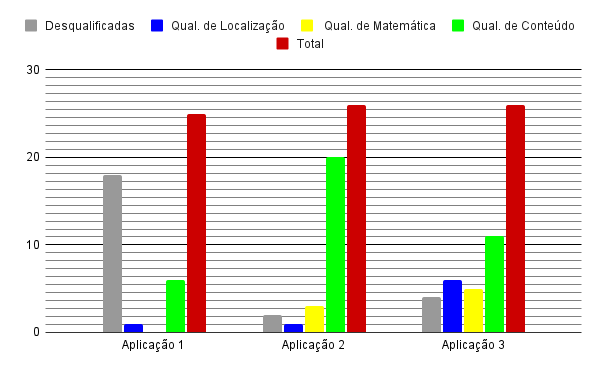
\includegraphics[width=1\textwidth]{fig/graficoDicasASA1.png}
\label{fig:dicasASA1}
\caption*{Fonte: Construção do Autor.}
\end{center}
\end{figure}

A  aplicação 1 (Apêndice \ref{ch:ASA1a1}) abordou o conteúdo de cinemática escalar. Durante as aulas, os alunos aprenderam sobre as convenções e construção dos sistemas de coordenadas, bem como o cálculo de velocidade e aceleração média. O conteúdo incluiu definições de deslocamento, distância percorrida e trajetória.

Foram realizados exercícios em sala de aula, muito semelhantes ao fornecido durante a  aplicação 1. Por esse motivo, supomos que os alunos não teriam dificuldade em resolver essa atividade.

Quando analisamos a Figura \ref{fig:dicasASA1}, podemos observar que a maioria dos questionamentos (72\%) feitos durante a aplicação 1 foram classificados como dúvidas desqualificadas. Isso indica que os alunos, ao encontrarem dificuldades, não sabiam como iniciar o processo para esclarecer suas dúvidas e prosseguir na RP.

A identificação de uma grande proporção de alunos solicitando dúvidas desqualificadas após a aplicação 1 revelou um quadro preocupante de dificuldades na compreensão do conteúdo. Diante desses resultados, o professor promoveu um diálogo com a turma para entender as razões por trás dessa dificuldade generalizada. A maioria dos alunos relatou não ter compreendido o conteúdo ministrado.

A constatação de que mais de um mês havia se passado desde o início do ano letivo quando a aplicação 1 foi realizada levou o professor a questionar os alunos sobre o quanto eles haviam estudado o conteúdo em casa nesse período. Surpreendentemente, muitos alunos admitiram não terem dedicado tempo suficiente aos estudos fora da sala de aula. Além disso, o professor percebeu que os alunos não o procuravam para tirar dúvidas, mesmo quando ele questionava em sala de aula sobre suas dificuldades. Esses aspectos levantaram preocupações sobre a necessidade de reforçar a importância do estudo individual e da busca ativa por esclarecimento de dúvidas para o progresso dos alunos.

Após o diálogo com os alunos, houve um compromisso por parte deles de se esforçarem mais no estudo individual, tanto na escola quanto em casa. Esse comprometimento refletiu diretamente nas aplicações 2 e 3 da ASA1, conforme ilustrado na Figura \ref{fig:dicasASA1}, onde o número de dúvidas desqualificadas diminuiu significativamente.

Dentro da aplicação 1, é importante mencionar os alunos que não solicitaram dicas ao professor durante a resolução das atividades. Nesse contexto, observou-se que 4 alunos optaram por não buscar ajuda, e, preocupantemente, apenas 1 desses estudantes conseguiu resolver corretamente a questão proposta.

De fato, a ausência de solicitação de dicas por parte de alguns alunos durante a resolução das atividades pode ser um indicativo de diferentes problemas. Como mencionado, isso pode sugerir que o aluno não tem clareza sobre como abordar o problema, pode demonstrar falta de interesse ou motivação para resolver a questão, ou até mesmo uma possível confiança excessiva em suas habilidades que leva a erros na resolução. Essas questões são preocupantes, pois podem impactar negativamente o desempenho do aluno e sua aprendizagem. 

Na aplicação 2 (Apêndice \ref{ch:ASA1a2}), trabalhamos especificamente o conceito de movimento retilíneo uniforme, considerando as dificuldades que os alunos tiveram com o conceito de velocidade na aplicação 1. Nosso objetivo era analisar os progressos dos alunos, inclusive no compromisso de estudarem em casa, por meio dessa abordagem mais focada.

Como já mencionado anteriormente, o número de dicas desqualificadas reduziu em relação à aplicação 1. No entanto, nessa etapa, surgiram dúvidas relacionadas tanto a conceitos matemáticos quanto a conteúdo específico da Física.

As dúvidas de origem Matemática estavam relacionadas à dificuldade dos alunos em montar uma função que relacionasse os dados fornecidos. Embora tenham sido apenas 3 dúvidas dessa natureza, é importante ficar atento ao fato de os alunos não conseguirem utilizar uma ferramenta matemática tão básica para a resolução dos problemas propostos.

As dúvidas de Conteúdo estavam relacionadas às formas de conversão de unidades e ao cálculo da distância a ser percorrida. Em muitos casos, essas perguntas surgiram ao mesmo tempo, o que indica uma dificuldade dos alunos em separar dois conceitos físicos distintos. A falta de clareza na compreensão desses conceitos pode ter contribuído para as dúvidas e dificuldades enfrentadas pelos alunos durante a resolução dos problemas. 

Nesta aplicação, constatamos que 6 alunos não solicitaram dicas ao professor, e, infelizmente, apenas 1 desses estudantes conseguiu acertar a questão. Esse mesmo aluno havia acertado a questão anterior na aplicação 1 sem precisar de dicas. 

A persistência do mesmo aluno em acertar a questão na aplicação 2, sem solicitar dicas ao professor, pode indicar que ele possui um bom domínio do conteúdo abordado e está mais confiante em suas habilidades. No entanto, é preocupante que os demais alunos que não solicitaram dicas também não tenham acertado a questão.

Na aplicação 3 (Apêndice \ref{ch:ASA1a3}), abordamos os conceitos de movimento retilíneo uniforme e movimento retilíneo uniformemente variado simultaneamente. Os alunos foram desafiados a resolver o problema que requeria uma boa compreensão desses tópicos, bem como o conceito de independência dos eixos no movimento.

Com base nas dificuldades enfrentadas nas atividades anteriores e na complexidade dos conceitos abordados, previmos que haveria uma distribuição mais equilibrada das solicitações de diferentes tipos de dicas na aplicação 3. Observando a Figura \ref{fig:dicasASA1} vemos que essa tendência se confirma.

É importante enfatizar a redução nas solicitações de dicas de Conteúdo e o aumento das dicas de Localização na aplicação 3. Esses dois tipos de dicas apresentaram a maior variação ao longo de todo o processo da ASA1.

Na aplicação 3, as dicas de Localização estão associadas ao fato de os alunos confundirem o movimento retilíneo uniforme com o movimento uniformemente variado. Além disso, esses mesmos estudantes apresentaram dúvidas de Conteúdo, demonstrando dificuldade em relacionar os dois tipos de movimento abordados na questão.

As dúvidas de Conteúdo foram, em sua maioria, associadas à forma e ao uso das equações dos movimentos. Apesar de receberem essas informações, os alunos continuavam apresentando dificuldades na resolução da questão.

Na última etapa da ASA1, tivemos 7 alunos que não solicitaram dicas. Dos alunos que não pediram dicas, 2 acertaram a questão. Um dos alunos foi o mesmo que acertou sem dicas nas duas aplicações anteriores, enquanto o outro não havia solicitado dicas e também não havia acertado nenhuma questão anteriormente.

O progresso do aluno mesmo sem o uso de dicas na última aplicação é notável. Ao conversar com ele, o professor descobriu que o estudante estava passando por problemas pessoais que o afetaram no início do período letivo.

\begin{table}[ht]
\centering
\caption{Principais perguntas dos alunos durante a ASA1.} \label{tab:pergASA1}
\begin{tabular}{c|c}
\hline
\textbf{Pergunta} & \textbf{Classificação}\\ \hline
Como identifico o tipo de movimento? & Localização\\ 
Como inicio a resolução da questão? & Desqualificada \\ 
Como calculo a distância percorrida? & Conteúdo \\
Qual é a equação da velocidade média? & Conteúdo \\
O tempo total é a soma dos tempos de cada etapa? & Conteúdo \\
Qual a fórmula que uso para converter a unidade da velocidade? & Conteúdo \\
\hline
\end{tabular}
\caption*{Fonte: Construção do Autor.}
\end{table}


Por fim, na Tabela \ref{tab:pergASA1} temos alguns exemplos das perguntas que foram mais repetidas pelos alunos ao longo de todo o processo de aplicação da ASA1. Esses questionamentos recebem a mesma classificação que o tipo de dica utilizada para respondê-los.

\subsubsection{Considerações Gerais da ASA1} \label{subsubsec:asa1}

Até o momento, foram apresentadas as principais características de cada aplicação da ASA1. No entanto, para alcançar uma abordagem mais abrangente, é essencial realizar uma análise integrada das três aplicações, a fim de possibilitar avaliações de qualidade. Essa análise conjunta permitirá compreender o comportamento coletivo da turma, considerando os diferentes tipos de dicas solicitadas e o desempenho dos alunos ao longo do processo.

Inicialmente, é essencial discutirmos o conteúdo das folhas de resolução dos alunos, como mencionado anteriormente na Seção \ref{sec:asa}. Esse objeto de estudo está diretamente relacionado ao objetivo \ref{item:a}.

É importante destacar que as aplicações da ASA1 representaram as primeiras experiências dos alunos em RP de Física. Nesse contexto, não tínhamos expectativas de que as respostas estivessem inicialmente bem organizadas e estruturadas. O processo de aquisição de habilidades em RP demanda tempo e prática, e é natural que os estudantes enfrentem dificuldades iniciais na abordagem dessas questões.

A análise das folhas revelou que, ao longo do período letivo, a maioria dos estudantes ainda apresentava dificuldades em organizar suas ideias para as resoluções dos problemas. Esse cenário ficou evidente pelo aumento no número de dicas desqualificadas na aplicação 3, indicando que os alunos continuavam a enfrentar obstáculos para progredir na resolução das questões de forma autônoma.

\begin{figure}
    \centering
    \caption{Exemplo de Organização ASA1.}
    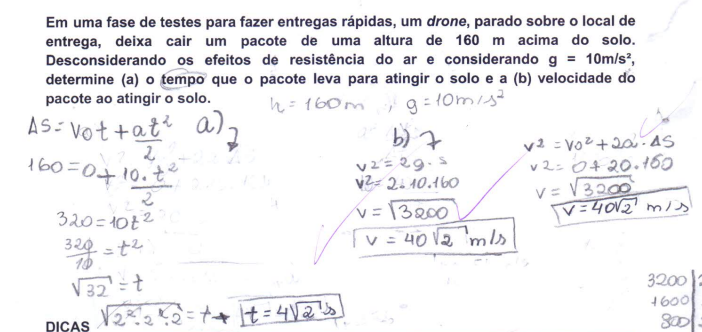
\includegraphics[width=1\textwidth]{fig/orgasa1.png}
    \caption*{Fonte: Extraído da produção dos Estudantes.}
    \label{fig:orgasa1}
\end{figure}

Os alunos que conseguiam estruturar suas ideias apresentaram respostas mais organizadas e claras em suas folhas de resolução (Figura \ref{fig:orgasa1}). Suas abordagens permitiam uma compreensão clara dos dados fornecidos, do questionamento apresentado e das estratégias adotadas para a resolução do problema. Esse padrão demonstra que esses alunos conseguiram articular de forma eficiente seus pensamentos, evidenciando uma maior capacidade de comunicação e coerência em suas respostas.

É relevante destacar que os alunos capazes de estruturar mais efetivamente seus pensamentos foram os mesmos que buscaram as dicas qualificadas. Esse fato evidencia uma correlação positiva entre a organização escrita e o raciocínio dos estudantes. Indica que os estudantes com resoluções mais bem organizadas também demonstraram uma propensão maior a solicitar orientações específicas, sugerindo uma abordagem mais sistemática e estratégica na RP.

Os alunos que foram capazes de resolver as questões mostraram-se proficientes em estruturar suas ideias e expressá-las por escrito. Eles começaram o processo anotando os dados e incógnitas relevantes e, em seguida, identificando quais partes do conteúdo estudado poderiam auxiliá-los na resolução do problema, avaliando a necessidade de solicitar dicas. 

A abordagem dos alunos ao resolver os problemas se assemelha significativamente aos procedimentos descritos por \citeonline{Pozo2009}. De fato, esses passos têm se mostrado uma forma eficiente de abordar a RP de Física. A organização das ideias e a identificação dos dados relevantes são elementos cruciais para um raciocínio claro e estruturado na busca de soluções em Física.

A análise das dicas fornecidas aos alunos foi escolhida para verificar o objetivo \ref{item:b}, uma vez que essas dicas foram categorizadas em quatro tipos distintos, conforme descrito na Seção \ref{sec:asa}. Essa abordagem permitiria identificar em quais momentos as ajudas foram mais relevantes, fornecendo informações sobre os pontos em que os estudantes apresentaram maior dificuldade e necessidade de orientação adicional.

Durante a realização da ASA1, um total de 77 dicas foram fornecidas aos alunos. Dessas dicas, 24 foram classificadas como desqualificadas, 8 como dicas de Localização, 8 de Matemática e 37 de Conteúdo. 

As expectativas iniciais apontavam para uma maior frequência de solicitações de dicas de Matemática, devido às dificuldades decorrentes da Pandemia. No entanto, observou-se que as dicas mais solicitadas pelos alunos foram as de Conteúdo e as classificadas como desqualificadas.

A análise dos resultados e as observações do professor indicam que os alunos enfrentaram uma maior dificuldade na compreensão das questões propostas. A Figura \ref{fig:difasa1} exemplifica a dificuldade de alguns alunos. Essa dificuldade foi evidenciada pelo fato de que, na maioria dos casos, os estudantes não conseguiram avançar para a etapa de aplicação dos conhecimentos e procedimentos matemáticos na resolução dos problemas. 

\begin{figure}
    \centering
    \caption{Dificuldade de resolução -  ASA1.}
    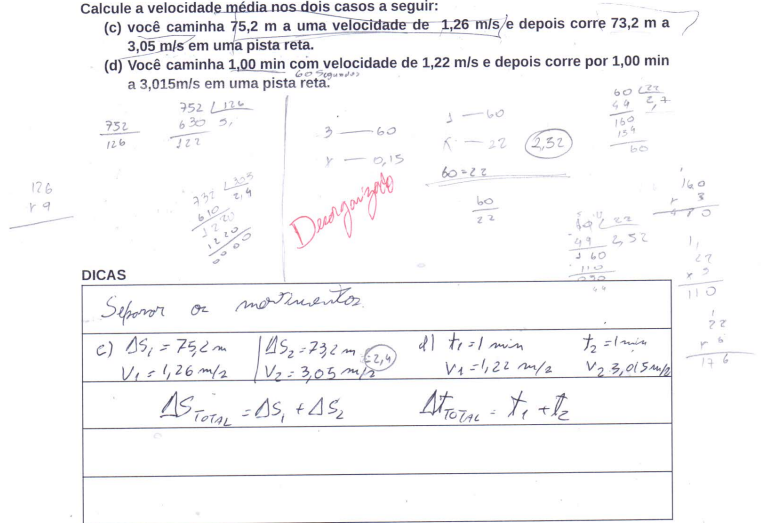
\includegraphics[width=1\textwidth]{fig/difasa1.png}
    \caption*{Fonte: Extraído da produção dos Estudantes.}
    \label{fig:difasa1}
\end{figure}

Esse cenário pode estar relacionado, também, às condições adversas causadas pela Pandemia, o que pode ter impactado negativamente a habilidade de leitura e interpretação dos enunciados pelos alunos. Essa dificuldade básica de leitura e interpretação das questões pode ter contribuído para as maiores solicitações de dicas desqualificadas durante a ASA1.

Com base na análise dos resultados da ASA1, podemos afirmar que, em relação ao objetivo \ref{item:b}, as etapas de RP que mais demandaram auxílio foram aquelas em que os alunos não conseguiam prosseguir na resolução e as que envolviam conhecimento específico de Física. Notavelmente, a falta de estudo por parte dos alunos, conforme evidenciado pelos relatos do Professor, parece estar diretamente relacionada à necessidade de auxílio nesses momentos.

Analisar a evolução temporal dos alunos na competência de Resolução de Problemas (objetivo \ref{item:c}) foi impossibilitado devido ao baixo desempenho dos mesmos. De fato, apenas alguns alunos conseguiram demonstrar um processo evolutivo representativo ao longo das atividades.

Apenas um único aluno conseguiu resolver todas as questões, sem o auxílio de dicas, o que inviabilizou a constatação de um processo evolutivo significativo. A maioria dos alunos oscilava entre os tipos de dicas solicitadas, sem obter sucesso nas resoluções, o que gerou preocupação nos pesquisadores. 

As atividades propostas eram similares às realizadas em sala de aula, indicando que os alunos não estavam estudando mesmo após o diálogo com a turma. O professor não percebeu movimentações por parte dos alunos para tirar dúvidas, tanto em aula quanto fora dela, reforçando a possível falta de empenho na busca pelo aprendizado.

Devido ao baixo desempenho dos alunos e à falta de progresso significativo durante as aplicações, não foi possível estabelecer quais formas de ajuda se tornaram mais eficientes, conforme o objetivo \ref{item:d}. Além disso, não houve oportunidades de auxiliar a turma fora das aplicações, o que dificultou ainda mais a avaliação da eficácia das dicas fornecidas. Os alunos também pareciam ter dificuldade em entender ou fazer uso das dicas. 

A última ferramenta utilizada para a análise das aplicações foi um questionário\footnote{\textbf{Pergunta 1 -} Sinto que os problemas presentes nas Atividades de Sala de Aula possuíam um grau de dificuldade similar aos problemas presentes no livro e nos realizados em sala de aula.\\ \textbf{Pergunta 2 -} Sinto que as Atividades de Sala de Aula são uma boa maneira de verificar meus conhecimentos e aprendizagens de Física.\\ \textbf{Pergunta 3 -} Sinto que as dicas presentes nas Atividades de Sala de Aula podem me auxiliar a resolver o problema quando não consigo prosseguir.\\ \textbf{Pergunta 4 -} Sinto que consigo entender melhor minhas dificuldades após a realização das Atividades de Sala de Aula.\\ \textbf{Pergunta 5 -} Considero que o número de Atividades de Sala de Aula poderia ser maior ao longo do trimestre.} (Apêndice \ref{ch:questASA}), o qual foi respondido de forma anônima e não obrigatória pelos alunos. Dos 16 alunos avaliados na ASA1, 10 deles responderam ao questionário, o que representa 62,5\% dos participantes.

\begin{table}[ht]
\centering
\caption{Respostas da ASA1 ao questionário final.} \label{tab:questASA1}
\begin{tabular}{ccccc}
\hline
\textbf{Pergunta 1} & \textbf{Pergunta 2} & \textbf{Pergunta 3} & \textbf{Pergunta 4} & \textbf{Pergunta 5} \\ \hline
5 & 4 & 5 & 3 & 4 \\ 
3 & 4 & 4 & 3 & 3 \\ 
3 & 4 & 4 & 2 & 5 \\ 
5 & 5 & 5 & 5 & 4 \\ 
4 & 5 & 5 & 5 & 5 \\ 
5 & 4 & 5 & 4 & 5 \\ 
4 & 5 & 1 & 1 & 5 \\ 
3 & 3 & 5 & 1 & 4 \\ 
4 & 3 & 1 & 1 & 5 \\ 
2 & 5 & 5 & 3 & 2 \\ \hline
\end{tabular}
\caption*{Fonte: Construção do Autor.}
\end{table}

A Tabela \ref{tab:questASA1} apresenta as respostas obtidas para as 5 perguntas, seguindo o padrão de escala Likert \cite{dalmoro}. Ao analisarmos as percepções dos alunos por meio do questionário, podemos obter uma melhor compreensão dos pontos positivos e negativos do processo até o momento. Isso nos permitirá identificar as áreas que precisam ser aprimoradas.

A primeira pergunta do questionário analisa a dificuldade das questões apresentadas na ASA. A maioria dos alunos concordou, ao menos parcialmente, que as questões eram tão difíceis quanto as apresentadas em aula. Essa concordância corrobora a informação fornecida pelo Professor de que os alunos não estavam dedicando o tempo necessário aos estudos, o que os impedia de resolver questões similares às já trabalhadas.

Os alunos também concordaram com a afirmação de que a ASA é uma boa maneira de verificar os conhecimentos de Física (pergunta 2). Eles reconhecem que, mesmo que as questões possam ser mais desafiadoras, a abordagem da ASA é uma alternativa válida em comparação com as provas tradicionais.

Quando questionados sobre a eficiência das dicas (pergunta 3), 80\% dos alunos que responderam concordaram que elas foram úteis. Entretanto, os outros 20\% discordaram totalmente da afirmação. É importante considerar que alguns alunos podem ter enfrentado dificuldades externas ao conteúdo de Física, o que pode ter impactado a percepção sobre a eficácia das dicas. Diante disso, é necessário repensar as estratégias das dicas para que mais alunos se sintam confortáveis ao fazer uso delas.

Uma observação importante, embora não surpreendente, é que a maioria dos alunos relatou não conseguir compreender melhor suas dificuldades após as aplicações da ASA (pergunta 4). Isso pode estar diretamente relacionado ao fato de que, nesta turma específica, os alunos enfrentaram dificuldades em fazer uso efetivo das dicas fornecidas durante o processo.

Observamos ainda que, em muitos casos, os alunos tinham receio de solicitar ajuda devido à redução no valor máximo da atividade. No entanto, parece que eles não percebiam que, caso não conseguissem resolver a questão, seu resultado seria ainda pior. Essa hesitação pode ter contribuído para a menor utilização das dicas e, consequentemente, para o menor progresso nas resoluções das questões.

Surpreendentemente, 80\% dos alunos responderam que poderiam ser realizadas mais aplicações da ASA ao longo do período letivo (pergunta 5). É importante considerar que o número de intervenções já foi elevado, uma vez que foram realizadas 3 aplicações ao invés de uma única prova. A opinião dos alunos sugere que eles perceberam os benefícios das aplicações e se sentiram mais confortáveis com esse formato de avaliação.

As respostas dos alunos nas observações e reclamações acerca do modelo das ASA (pergunta dissertativa) mostraram-se limitadas, uma vez que alguns alunos não pareceram compreender totalmente a proposta da pergunta. Alguns dos participantes deixaram esse espaço em branco, o que pode indicar falta de clareza sobre como abordar o assunto ou simplesmente a ausência de reclamações significativas. 

As respostas, em sua maioria, foram relacionadas às aulas do Professor, e não às atividades em si. As reclamações estavam relacionadas ao tempo dedicado pelo Professor em sala de aula para a explicação de cada tópico do conteúdo. Em resposta a essas preocupações, houve um diálogo com a turma, onde o Professor explicou que o conteúdo a ser trabalhado é muito extenso para a quantidade de períodos letivos semanais, o que limita o tempo disponível para aprofundar cada tópico.

Foi reforçada a importância dos estudantes dedicarem tempo ao estudo em casa e enviarem suas dúvidas para o Professor. Esse processo de comunicação e apoio fora das aulas presenciais foi enfatizado desde o início do ano letivo como uma forma de proporcionar um melhor aproveitamento do conteúdo e esclarecer as dificuldades enfrentadas pelos alunos. 

Com base nas informações obtidas pelo questionário e nas anotações e observações do Professor, não foi possível identificar uma manutenção do interesse na resolução de problemas ao longo do trimestre (objetivo \ref{item:e}). De fato, podemos afirmar que, de modo geral, essa turma não demonstrou interesse em buscar meios para desenvolver suas habilidades nessa área. O fato de não buscarem ajuda, tanto em sala de aula quanto fora dela, e a falta de evolução significativa na resolução dos problemas sugerem uma falta de engajamento e motivação por parte dos alunos em aprimorar sua competência de resolução de problemas de Física.

\subsection{ASA2} \label{subsec:asa2}


A ASA2 contou com a participação de 21 alunos, de um total de 26 matriculados na turma de 2º ano do Ensino Médio (ver Tabela \ref{tab:basicoASA}). Os critérios para escolha da turma e exclusão de determinados alunos foram os mesmos utilizados na ASA1.

O Professor já havia ministrado a disciplina de Física para essa turma no 1º ano do Ensino Médio. Antes disso, os estudantes passaram pelo 8º ano do Ensino Fundamental em formato remoto, devido à Pandemia, e pelo 9º ano de forma híbrida.

Da mesma forma que ocorreu na turma da ASA1, houve uma flexibilização das faltas na escola quando o Professor lecionou pela primeira vez para a turma. Isso ocorreu devido às dificuldades de adaptação dos alunos no retorno ao sistema presencial, e alguns deles estavam em risco de abandonar os estudos.

A flexibilização das faltas foi essencial para evitar a evasão escolar. No entanto, durante o processo de aplicação da ASA2, ainda foram percebidos resquícios da dificuldade de adaptação por parte de alguns estudantes. Essa situação resultou em defasagens nos conhecimentos dos alunos, impactando o desenvolvimento das atividades.

Durante o 1º ano, o Professor assumiu a turma na metade do ano letivo e constatou que o conteúdo programático estava atrasado. Como resultado, não foi possível abranger todo o conteúdo previsto para o 1º ano do Ensino Médio. Essa lacuna na formação dos estudantes tem impacto direto ao gerar dificuldades adicionais no processo de aprendizagem dos estudantes.

Durante a ASA2, considerando as dificuldades pré-existentes dos alunos com operações matemáticas e interpretação de texto, era esperado observar uma maior quantidade de solicitações de dicas desqualificadas e de Matemática. Esses aspectos poderiam impactar diretamente o desempenho dos estudantes nas atividades propostas, uma vez que essas habilidades são fundamentais para a RP de Física. 

\begin{figure}[ht]
\begin{center}
\caption{Gráfico das dicas solicitadas ao longo da ASA2.}
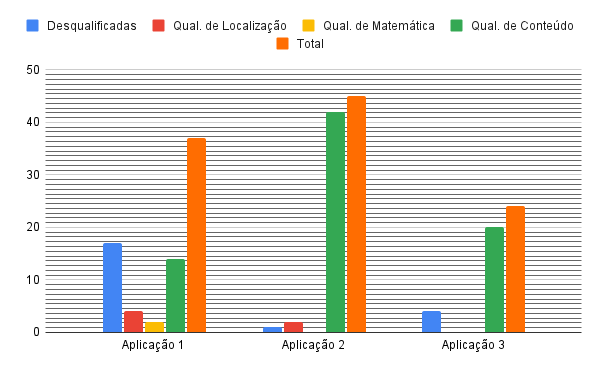
\includegraphics[width=1\textwidth]{fig/graficoDicasASA2.png}
\label{fig:dicasASA2}
\caption*{Fonte: Construção do Autor.}
\end{center}
\end{figure}

Ao longo da ASA2, foram conduzidas 3 aplicações que estão disponíveis no Apêndice \ref{apendice:asa2}. A Figura \ref{fig:dicasASA2} apresenta um gráfico ilustrando a quantidade e o tipo de dicas fornecidas aos alunos durante cada uma dessas três atividades. Essas informações são relevantes para entendermos o auxílio que os estudantes buscaram ao enfrentar os problemas propostos e para analisar os padrões de dificuldades encontrados pelos alunos.

A aplicação 1 (Apêndice \ref{ch:ASA2a1}) consistia em um problema de conversão de escalas térmicas. Durante as aulas expositivas, o Professor ensinou os alunos a realizar a conversão entre as três escalas térmicas mais comuns - Celsius, Kelvin e Fahrenheit. Além disso, foi demonstrado como criar uma equação geral de conversão entre duas escalas de temperatura quaisquer, proporcionando aos estudantes ferramentas para resolver problemas envolvendo esse tipo de conversão.

Esperávamos que os alunos não encontrassem dificuldades significativas no processo de resolução da aplicação 1. No entanto, caso solicitassem dicas, esperávamos que fossem do tipo qualificadas, possivelmente relacionadas a Matemática ou ao Conteúdo (específico da conversão de escalas térmicas). A expectativa das dicas de Matemática decorria do histórico de dificuldades da turma nessa área, enquanto as de Conteúdo poderiam surgir caso os alunos não se lembrassem de algum detalhe relevante para realizar a conversão.

Ao analisarmos a Figura \ref{fig:dicasASA2}, percebemos que nossas expectativas em relação às dicas de Conteúdo se confirmaram. No entanto, ao invés de termos um número elevado de estudantes com dificuldades em Matemática, a maioria deles enfrentou dificuldades no início da resolução do problema, o que resultou na solicitação de dicas desqualificadas. 

Isso indica que a turma enfrentou obstáculos no início do processo de resolução, possivelmente relacionados à compreensão do enunciado ou à identificação dos dados relevantes para a conversão de escalas térmicas. Esses obstáculos revelam que a dificuldade previamente mencionada em interpretação de texto dos estudantes pode ser mais desafiadora do que inicialmente esperado.

Dos 21 alunos avaliados, 5 não solicitaram nenhuma dica durante a aplicação 1. Dentre esses, 2 conseguiram resolver a questão. Um deles já era esperado, sendo reconhecido como um bom aluno e participante assíduo de provas e olimpíadas estudantis, frequentemente recebendo premiações.

O outro estudante que acertou a questão foi um dos que quase abandonou a escola. Ele relatou ao Professor que havia começado a estudar e se dedicaria a isso. Esses casos se repetirão ao longo da ASA2, tornando relevante a antecipação dessa informação para evitar repetições posteriores.

O processo da aplicação 2 (Apêndice \ref{ch:ASA2a2}) abordou os conceitos de transferência de calor e mudança de estado físico. Em sala de aula, o Professor já havia resolvido questões semelhantes com os alunos, mas a principal diferença nesta aplicação foi a necessidade de realizar duas mudanças de estado físico, em contraste com as questões abordadas anteriormente, que envolviam apenas uma mudança.

Essa diferença foi estabelecida com o propósito de transformar o que seria um simples exercício, uma vez que os alunos já estavam familiarizados com a resolução, em um desafio que exigiria a aplicação de conhecimentos prévios. Nesse contexto, esperávamos que, de maneira geral, a turma não precisasse de muitas dicas, com exceção talvez da parte Matemática, em virtude das características prévias dos alunos, e da parte de Conteúdo, devido às diferenças em relação ao que já haviam aprendido anteriormente.

A análise dos tipos de dicas utilizados confirmou nossas previsões. A grande maioria das dicas solicitadas pelos alunos foram de Conteúdo. Especificamente, as perguntas mais frequentes referiam-se às equações do calor sensível, do calor latente e como calcular o calor total no processo.

Isso indica que, apesar dos alunos não terem memorizado as equações, eles tinham conhecimento do procedimento necessário para resolver o problema, e as dicas foram úteis nesse processo. Infelizmente, a maioria dos alunos não conseguiu concluir a resolução corretamente ou resolveu de forma equivocada.

Nesses casos, os alunos acabaram cometendo erros em operações básicas matemáticas ou não conseguiram responder corretamente à pergunta. Isso evidencia novamente a dificuldade dos alunos na interpretação de texto e na execução de operações matemáticas. Essas habilidades são fundamentais para a resolução adequada de problemas, e a identificação dessas dificuldades destaca a necessidade de focar no desenvolvimento dessas competências ao longo do processo educacional.

A identificação de 5 alunos que não pediram dicas durante a aplicação 2, sendo que 3 deles erraram a questão, é um indicativo importante sobre o engajamento e a disponibilidade desses estudantes para dedicarem-se aos estudos de Física. O fato de estarem participando de aulas no contra turno e outras atividades extracurriculares pode estar impactando negativamente o tempo disponível para o estudo individual, prejudicando assim o seu desempenho nas atividades propostas.

Durante o processo da aplicação 3 (Apêndice \ref{ch:ASA2a3}), trabalhamos novamente a transferência de calor, mas dessa vez, utilizando mais conceitos da termometria em comparação à atividade anterior. Essencialmente, abordamos os mesmos fenômenos físicos, porém com enfoques distintos.

Ao analisar a Figura \ref{fig:dicasASA2}, observamos uma redução significativa no número total de dicas solicitadas em relação às duas outras aplicações. Além disso, notamos que essas dicas foram, em sua maioria, do tipo Conteúdo.

A redução no número total de dicas se deve, possivelmente, ao fato de termos mais alunos que não solicitaram dica nenhuma, totalizando 8. Além disso, as dicas de Conteúdo mostram que os alunos não se preocuparam em memorizar as equações, já que poderiam solicitar ajuda, mas mantiveram o foco em entender os procedimentos para saber como aplicar as dicas.

Outra observação positiva que podemos fazer acerca desta aplicação é o fato de mais estudantes terem conseguido completar a resolução. Infelizmente, nem todos acertaram completamente, apresentando erros matemáticos ou alguma falha procedimental. No entanto, eles se esforçaram para fazer o máximo possível, onde mais de 60\% da turma não abandonou o processo de resolução.

O empenho e a dedicação dos alunos em permanecer no processo de resolução de problemas refletem uma atitude positiva. Essa perseverança evidencia um interesse genuíno em aprimorar suas habilidades de RP e a disposição para enfrentar os desafios que surgem durante o processo.

A atitude dos alunos em não desistir diante de erros e falhas é positiva e motivadora, demonstrando engajamento no processo de aprendizado e disposição para enfrentar os desafios da RP de Física. Essa postura é essencial para o desenvolvimento das habilidades na RP e para o progresso dos estudantes no contexto educacional.

\begin{table}[ht]
\centering
\caption{Principais perguntas dos alunos durante a ASA2.} \label{tab:pergASA2}
\begin{tabular}{c|c}
\hline
\textbf{Perguntas} & \textbf{Classificação}\\ \hline
O que eu faço com essas duas escalas? & Desqualificada \\
Preciso utilizar os valores do enunciado para resolver a questão? & Desqualificada \\
Pode me ajudar a montar o diagrama de fases? & Conteúdo \\
Qual o modelo da equação de conversão? & Conteúdo \\
Quais são as equações do calor? & Conteúdo\\
\hline
\end{tabular}
\caption*{Fonte: Construção do Autor.}
\end{table}

Na Tabela \ref{tab:pergASA2} trazemos algumas das perguntas que mais foram realizadas pelos estudantes ao longo do processo da ASA2. Nela também vemos a classificação dessas perguntas, em acordo com os critérios adotados para a classificação das respostas.

\subsubsection{Considerações Gerais da ASA2} \label{subsubsec:asa2}

Nesta etapa, conduziremos uma análise geral da ASA2, abordando aspectos das três aplicações. Para tal, utilizaremos as ferramentas de pesquisa descritas na Seção \ref{sec:asa}, conectando-as aos objetivos deste estudo.

A primeira ferramenta de análise que abordaremos são as folhas de resposta dos alunos. Nossa expectativa era encontrar as questões resolvidas de forma ordenada e organizada, além de observar o uso de desenhos e diagramas durante o processo de resolução. Essa ferramenta está conectada ao objetivo \ref{item:a}, que visa compreender como os alunos abordam a RP de Física.

Compreendemos que essa expectativa se baseia no conhecimento prévio sobre as condições da turma, considerando que eles já tiveram experiência prévia com a disciplina de Física. Apesar das lacunas de conhecimento existentes, os alunos demonstram esforço na busca por melhorar seus resultados e habilidades de RP.

Ao analisarmos as folhas de resposta, constatamos que a maioria dos estudantes confirmou nossas expectativas. Embora alguns precisassem de ajuda para lembrar como iniciar o processo de resolução de problemas, ao resolverem a questão, seguiam sempre uma estrutura lógica consistente.

A estrutura lógica observada consistia em três etapas principais: identificação e anotação das informações e objetivos da questão, criação de um esboço ou diagrama do processo envolvido, e posteriormente, traçar e implementar uma estratégia para a resolução. Essa abordagem se assemelha ao processo descrito por \citeonline{Pozo2009}, o que indica uma similaridade na forma de abordar e resolver problemas de Física entre os alunos da ASA2 e os estudantes da ASA1.

Ao longo das três aplicações, a turma utilizou um total de 106 dicas. Dentre essas, 22 foram consideradas desqualificadas, 6 de Localização, apenas 2 de Matemática e 76 de Conteúdo. As dicas desqualificadas tiveram como objetivo lembrar os alunos de analisar as informações presentes no problema e reforçar a possibilidade de criar diagramas para auxiliar na interpretação e resolução dos problemas.

Constatamos que, ao contrário do que inicialmente imaginávamos, os alunos não solicitaram muitas dicas de Matemática durante as aplicações. No entanto, durante a análise do processo, observamos que as dificuldades em matemática básica ainda persistem entre os estudantes (Figura \ref{fig:mtmasa2}). Afinal, foram identificados erros em operações simples, como multiplicação de números inteiros. 

\begin{figure}[ht]
\begin{center}
\caption{Exemplo de dificuldade em Matemática ao longo da ASA2.}
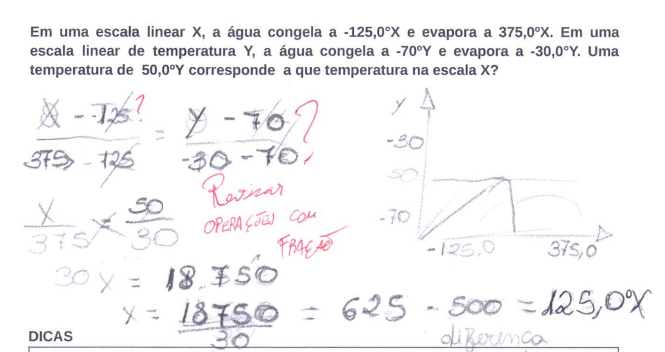
\includegraphics[width=1\textwidth]{fig/mtmasa2.png}
\label{fig:mtmasa2}
\caption*{Fonte: Extraído da produção dos Estudantes.}
\end{center}
\end{figure}


Nesse contexto, emerge a hipótese de que os alunos possam não estar suficientemente atentos durante o processo de resolução. Além disso, aqueles que enfrentaram dificuldades e não avançaram significativamente na resolução podem não ter solicitado dicas de Matemática por não terem alcançado uma etapa em que essa forma de auxílio fosse necessária.

No que diz respeito às dicas de Conteúdo, que foram a maioria nesta aplicação, é importante analisar o contexto geral em que foram solicitadas. Os alunos, após conseguirem estruturar o processo de resolução, enfrentavam dificuldades em recordar as equações necessárias. Nessas situações, eles faziam questionamentos direcionados, solicitando, por exemplo, uma equação pelo nome da variável que buscavam. 

De fato, os alunos demonstraram um bom discernimento sobre o que procurar para progredir na resolução da questão. É provável que, nessas situações, se houvesse um formulário na atividade com as informações relevantes, eles não teriam necessitado solicitar essa dica específica, pois teriam acesso direto às informações necessárias para avançar na resolução - como mostrado na Figura \ref{fig:dicasasa2}. Isso evidencia, novamente, que os estudantes estavam mais focados em compreender o processo de resolução e em como aplicar as dicas de Conteúdo de forma adequada, em vez de depender apenas da memorização das equações.

\begin{figure}[ht]
\begin{center}
\caption{Exemplo de Dicas fornecidas ao longo da ASA2.}
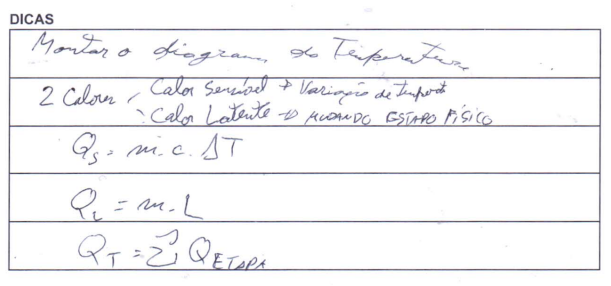
\includegraphics[width=1\textwidth]{fig/dicasasa2.png}
\label{fig:dicasasa2}
\caption*{Fonte: Extraído da produção dos Estudantes.}
\end{center}
\end{figure}

Concluindo, constatamos que, em relação ao objetivo \ref{item:b}, a etapa que mais demandou auxílio durante o processo de Resolução de Problemas foi a de Conteúdo, seguida da etapa inicial em que as dicas desqualificadas guiaram o processo. No entanto, é igualmente importante observar as dicas de Matemática, que também possuem potencial de serem mais solicitadas, mediante avanço no processo resolutivo.

Durante o processo da ASA2, pudemos observar uma evolução no processo de Resolução de Problemas (objetivo \ref{item:c}) por parte dos alunos. Ao analisarmos a Figura \ref{fig:dicasASA2}, percebemos uma oscilação na quantidade total de dicas utilizadas ao longo das aplicações.

Durante o período entre a aplicação 1 e a aplicação 2, observamos um aumento significativo no número total de dicas utilizadas pelos alunos. Esse aumento se refletiu, principalmente, na conversão de dicas desqualificadas para dicas de Conteúdo. Ou seja, os alunos passaram a solicitar menos dicas de caráter genérico e mais dicas específicas relacionadas ao conteúdo das questões.

Essa mudança indica um progresso na capacidade dos alunos de compreender e aplicar os processos envolvidos na RP. Ao se depararem com desafios mais complexos, eles demonstraram uma maior habilidade em identificar quais informações eram necessárias para prosseguir e quais conceitos precisavam ser aplicados para chegar à solução.

A redução significativa no número total de dicas utilizadas entre a aplicação 2 e a aplicação 3 reflete o aprimoramento das habilidades dos alunos em RP. Eles se tornaram mais conscientes do processo de RP e demonstraram uma maior autonomia na resolução das questões, necessitando de menos auxílio ao longo do caminho.

O estilo de dicas utilizado pelos alunos se manteve consistente, com uma ênfase maior em solicitar dicas de Conteúdo, o que indica que eles estavam buscando compreender e aplicar os conceitos específicos das questões.

Essa evolução positiva na resolução dos problemas mostra que os alunos assimilaram os conceitos trabalhados durante as atividades anteriores e adquiriram uma maior compreensão das estratégias para solucionar as questões propostas. Ao colocar em prática o que aprenderam, eles demonstraram um melhor domínio das habilidades de RP, o que contribuiu para o êxito alcançado na aplicação 3.

Através das observações feitas pelos alunos durante os processos de aplicação, percebemos uma preferência clara em relação ao formato das dicas (objetivo \ref{item:d}). Essa conclusão foi obtida após os alunos relatarem que certas explicações não foram compreendidas no momento em que as dicas foram fornecidas.

Durante as aplicações, ao fornecer dicas desqualificadas, observamos que os alunos demonstravam preferir um estilo em que lhes fossem apresentados apontamentos sobre como prosseguir. Por exemplo, na aplicação 1 (Apêndice \ref{ch:ASA2a1}), os estudantes pareceram entender melhor a informação quando lhes era dito: "Você sabe que existem 2 escalas de Temperatura e precisa relacioná-las. Como fazer isso?"

Ao receber essa informação, os alunos eram levados a refletir sobre o assunto. Na maioria dos casos, esse tipo simples de dica, seguida de um questionamento, levava os estudantes a progredir. Esse progresso ocorria de duas formas: através da resolução do problema ou da formulação de uma nova pergunta, geralmente de forma Qualificada.

Além das dicas desqualificadas, vamos abordar a eficiência das dicas de Conteúdo, uma vez que constituíram a maior parte das orientações fornecidas. Nesse contexto, identificamos duas formas distintas de Conteúdo: teoria e prática.

As dicas de teoria abordavam conceitos fundamentais e equações relacionadas ao problema, enquanto as dicas de prática forneciam orientações mais diretas sobre como aplicar esses conceitos na resolução específica da questão.

Quando a dúvida dos alunos estava relacionada à lembrança de uma equação, foi mais eficiente e útil fornecer-lhes diretamente a equação necessária. Dessa forma, eles puderam aplicar as informações que já haviam extraído e prosseguir com mais facilidade em seu desenvolvimento no processo de resolução.

Quando a dúvida dos alunos estava relacionada aos conceitos da matéria, foi necessário fornecer uma pequena explicação sobre aquela parte específica do conteúdo. Por exemplo, na aplicação 2 (Apêndice \ref{ch:ASA2a2}), os alunos precisavam calcular o calor total em um processo de mudança de fase. Muitos deles apresentaram dúvidas sobre como aplicar os calores sensível e latente nessa situação.

Nesse contexto, a dica foi fornecida na forma de uma explicação rápida, como "O calor sensível será utilizado quando houver mudança de estado físico." Essa abordagem permitiu que os alunos compreendessem como utilizar os conceitos de calor sensível e latente na resolução do problema específico e avançassem em sua resolução com maior clareza e segurança.

\begin{table}[H]
    \centering
    \caption{Respostas da ASA2 ao questionário final.}\label{tab:questASA2}
    \begin{tabular}{ccccc}
    \hline
        \textbf{Pergunta 1} & \textbf{Pergunta 2} & \textbf{Pergunta 3} &\textbf{Pergunta 4} & \textbf{Pergunta 5} \\ \hline
        1 & 1 & 2 & 1 & 1 \\ 
        1 & 4 & 4 & 4 & 1 \\ 
        2 & 5 & 5 & 2 & 1 \\ 
        1 & 4 & 5 & 4 & 2 \\ 
        3 & 1 & 2 & 1 & 1 \\ 
        1 & 1 & 2 & 1 & 1 \\ 
        1 & 4 & 4 & 4 & 1 \\ 
        2 & 1 & 1 & 1 & 1 \\ 
        1 & 2 & 2 & 1 & 2 \\ 
        2 & 3 & 4 & 3 & 2 \\ 
        3 & 4 & 5 & 2 & 4 \\ 
        3 & 4 & 5 & 3 & 1 \\ 
        3 & 5 & 5 & 3 & 3 \\ 
        2 & 4 & 2 & 3 & 2 \\ 
        1 & 1 & 1 & 1 & 1 \\ 
        2 & 4 & 3 & 4 & 3 \\ 
        3 & 2 & 5 & 4 & 5 \\ 
        3 & 1 & 4 & 1 & 3 \\ 
        1 & 5 & 3 & 5 & 5 \\ 
        3 & 1 & 2 & 4 & 2 \\ \hline
    \end{tabular}
    \caption*{Fonte: Construção do Autor.}
\end{table}

A Tabela \ref{tab:questASA2} apresenta os resultados obtidos para as cinco primeiras perguntas do questionário (Apêndice \ref{ch:questASA}) aplicado ao fim da ASA2. Assim como realizado para a ASA1, procederemos com a análise e discussão das respostas para cada pergunta de forma individual.

O alto índice de participação dos alunos no questionário da ASA2, com 20 dos 21 alunos avaliados respondendo, é um fator positivo a ser destacado. Isso reforça o perfil engajado da turma, demonstrando que os estudantes estão interessados em contribuir com a avaliação do processo de RP e em compartilhar suas percepções sobre as atividades desenvolvidas.

Essa atitude pró-ativa dos alunos em participar do questionário mostra que eles estão dispostos a fornecer \textit{feedbacks} relevantes para o aprimoramento do processo de ensino-aprendizagem. Além disso, ao expressarem suas opiniões e experiências, os alunos podem contribuir para que o professor compreenda melhor suas necessidades e dificuldades, auxiliando na identificação de pontos fortes e áreas de melhoria nas próximas aplicações da ASA ou em outras atividades pedagógicas.

Diferentemente das respostas obtidas na ASA1, aqui tivemos discordância quanto ao grau de dificuldade das questões durante as aplicações (pergunta 1). Ao compararmos as questões antes e depois da modificação para uso na ASA, conforme exemplificado na Tabela \ref{ref:questoes} na Seção \ref{sec:asa}, podemos inferir que os alunos podem não ter se familiarizado plenamente com o estilo de modificações nas questões durante a ASA2. Essa falta de familiaridade pode ter influenciado na percepção de dificuldade, levando a uma divergência nas respostas.

Houve uma divisão de opiniões na turma quanto à eficácia da ASA em avaliar os conhecimentos e aprendizagens de Física (pergunta 2). É importante lembrar que a ASA é uma abordagem diferenciada de avaliação, que visa estimular o desenvolvimento das habilidades de RP, indo além da simples memorização de conteúdos.

Os alunos que manifestaram dificuldades ou preferência por outro modelo de avaliação podem estar acostumados a formatos mais tradicionais, onde a ênfase é na memorização de fórmulas e conceitos, e a resolução de exercícios se assemelha a repetir fórmulas prontas. A ASA, por outro lado, busca incentivar a autonomia dos alunos, a capacidade de enfrentar desafios e a aplicação prática do conhecimento adquirido.

A divergência de opiniões dos alunos em relação à qualidade das dicas apresentadas na ASA é uma reflexão importante para aprimorar o processo (pergunta 3). O fato de alguns alunos não se sentirem confiantes ou convencidos da eficácia das dicas pode ter influenciado na utilização das mesmas ao longo da ASA.

Para melhorar a aceitação e efetividade das dicas, é necessário buscar alternativas que possam atender às diferentes necessidades dos alunos. Isso pode envolver a oferta de diferentes tipos de dicas, como exemplos detalhados, explicações mais aprofundadas ou até mesmo recursos visuais e práticos para auxiliar na compreensão dos conceitos.

A análise das respostas da pergunta 4 do questionário, que abordou a sensação de compreensão das próprias dificuldades após as aplicações da ASA, evidenciou, novamente, uma divisão de opiniões na turma. Os alunos que não demonstram confiança no processo das dicas provavelmente não experimentaram uma mudança significativa em sua percepção sobre suas próprias dificuldades na disciplina.

Essa divergência pode estar diretamente relacionada à eficácia percebida das dicas oferecidas durante as aplicações. Os estudantes que não se sentem confiantes na utilidade ou eficácia das dicas podem não ter vivenciado uma melhora substancial em sua compreensão das dificuldades enfrentadas no aprendizado da Física.

Essa constatação ressalta a importância de revisar e aprimorar o processo de fornecimento de dicas, visando torná-las mais efetivas e relevantes para atender às necessidades individuais dos alunos. Além disso, é fundamental considerar outros fatores que podem influenciar a percepção dos alunos sobre suas dificuldades, como a abordagem do conteúdo em sala de aula, o ambiente de aprendizagem e a motivação dos estudantes.

A análise da pergunta 5 do questionário evidencia que a maioria dos alunos discorda da possibilidade de mais aplicações ao longo do trimestre. Essa preferência é fundamentada na percepção de que eles valorizam mais as atividades realizadas em sala de aula e as aulas expositivas. A limitação de tempo durante as aulas, devido à realização das aplicações, pode ser um fator que contribui para essa preferência, uma vez que os estudantes desejam mais oportunidades de interação com o professor e atividades tradicionais em sala de aula para fortalecer o aprendizado. 

Ao analisar o interesse na Resolução de Problemas (RP) ao longo do trimestre (objetivo \ref{item:e}), podemos afirmar que houve, de fato, interesse por parte dos alunos. Apesar de discordarem dos meios utilizados, ou seja, das aplicações, todos os alunos fizeram o esforço de buscar resolver as questões apresentadas da melhor forma possível. Esse comportamento evidencia que eles se empenharam em enfrentar os desafios propostos e demonstraram interesse em desenvolver suas habilidades de RP, mesmo que as estratégias de avaliação não tenham sido totalmente satisfatórias para eles. Portanto, o interesse dos alunos pela RP se manteve presente ao longo do trimestre, mesmo com as discordâncias sobre as formas de avaliação.


\subsection{ASA3} \label{subsec:asa3}

A seleção da turma do 3º ano do Ensino Médio para esta etapa do estudo foi definida pelo fato de o autor deste trabalho ser o professor regente da turma. Além disso, o professor já havia lecionado para essa mesma turma no ano anterior, o que permitiu uma familiaridade maior com as características e o histórico de aprendizado dos alunos.

Com base na experiência anterior do professor com a turma do 3º ano do Ensino Médio e nas condições de ensino que os alunos enfrentaram no 1º ano do Ensino Médio (formato híbrido) e no 9º ano do Ensino Fundamental (formato remoto), sabíamos que eles poderiam apresentar dificuldades prévias em Matemática e Física. Essas dificuldades poderiam ser semelhantes às observadas na turma da ASA2, considerando a transição entre o Ensino Fundamental e o Ensino Médio e as adaptações ao ensino remoto e híbrido.

Durante a experiência de lecionar para a turma do 2º ano do Ensino Médio, o professor observou que existem dificuldades notórias em Matemática e Física. No entanto, ele também destaca que essa turma se destaca pelo empenho e dedicação aos estudos. Essa característica positiva dos alunos pode ser um fator motivador para enfrentar os desafios encontrados na disciplina e buscar melhorar suas habilidades de RP.

Com base nas características positivas observadas da turma durante o 2º ano do Ensino Médio, como o empenho e dedicação aos estudos, as expectativas em relação ao rendimento da turma durante a ASA3 são bastante otimistas. Acreditamos que os alunos possuirão uma postura ativa e comprometida no processo de RP em Física, buscando superar desafios e aprimorar suas habilidades.

Além disso, esperamos que os estudantes forneçam boas observações e \textit{feedbacks} sobre a experiência com a ASA3. A turma já possui uma relação de confiança com o professor, o que pode favorecer a abertura para expressar suas opiniões de forma construtiva. Essas observações serão valiosas para avaliar a efetividade das estratégias pedagógicas adotadas e para identificar possíveis melhorias no processo de resolução de problemas.

\begin{figure}[ht]
\begin{center}
\caption{Gráfico das dicas solicitadas ao longo da ASA3.}
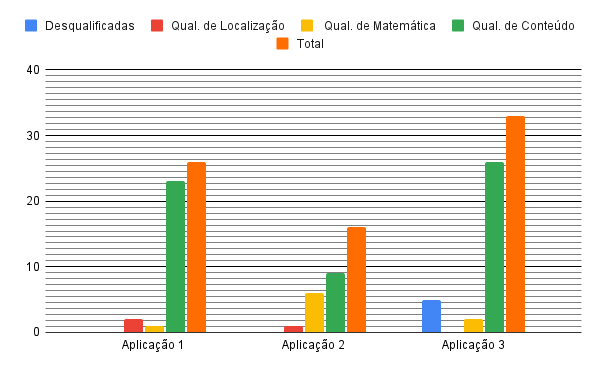
\includegraphics[width=1\textwidth]{fig/graficoDicasASA3.png}
\label{fig:dicasASA3}
\caption*{Fonte: Construção do Autor.}
\end{center}
\end{figure}

A turma do 3º ano do Ensino Médio, composta por 19 alunos, teve a participação de 14 estudantes avaliados durante o processo da ASA3. A exclusão de alguns alunos do estudo ocorreu pelos mesmos motivos já citados anteriormente, como questões de saúde, ausência na data da aplicação das atividades ou outros impedimentos que inviabilizaram a participação na ASA3.

A Figura \ref{fig:dicasASA3} apresenta a quantidade e o tipo de dicas fornecidas ao longo do processo da ASA3. É notável que há uma variação significativa no número total de dicas fornecidas em cada aplicação, o que nos leva a uma análise detalhada das razões por trás dessas oscilações.

Durante a aplicação 1 (Apêndice \ref{ch:ASA3a1}), foi trabalhada uma questão sobre carga elétrica. Nessa atividade, os alunos foram desafiados a calcular a quantidade de elétrons que deveriam ser retirados ou adicionados a um corpo para que ele assumisse uma carga elétrica específica.

Antes do início do processo das aplicações da ASA3, a turma foi informada sobre a necessidade de saber utilizar corretamente as sub e supra unidades de medida. Essa informação gerou preocupação entre os estudantes, que relataram ter dificuldades em memorizar esse tipo de informação. 

A decisão de enfatizar o uso correto das sub e supra unidades de medida foi motivada pelo entendimento de que a turma enfrentaria desafios em avaliações futuras, como Vestibulares e ENEM, onde informações específicas sobre essas unidades nem sempre são fornecidas. Além disso, é importante considerar que os níveis de exigência das questões podem variar ao longo do Ensino Médio.

Com base nas preocupações manifestadas pelos alunos, esperávamos observar um grande número de solicitações de dicas de Conteúdo, especialmente relacionadas às sub e supra unidades de medida. Ao contrário das aplicações anteriores, não tínhamos tanta expectativa em relação a solicitações de dicas de Matemática, já que os alunos não demonstraram preocupações específicas nessa área.

Analisando a Figura \ref{fig:dicasASA3}, podemos observar que houve apenas 1 solicitação de dica de Matemática. No entanto, contrariando nossas expectativas, os alunos demonstraram mais dificuldades na utilização dos conceitos matemáticos do que a quantidade de solicitações de dicas sugere. 

Essa discrepância pode ser um indicativo de que os alunos enfrentaram dificuldades matemáticas, mas talvez tenham relutado em pedir ajuda nessa área específica durante o processo de resolução das questões, ou, pior ainda, não tenham percebido que suas operações estavam equivocadas.

Dos alunos avaliados, 3 não solicitaram nenhuma dica. Observamos que esses alunos apresentaram dificuldades nos conceitos matemáticos, especificamente na inabilidade de operar com potências. Parece que eles preferiram não pedir ajuda durante o processo de resolução. Após a correção da atividade, o professor sugeriu que revisassem esse conteúdo, pois é fundamental para o desenvolvimento ao longo do ano letivo.

Nossa expectativa sobre as dúvidas de Conteúdo foi confirmada. Além de serem a maioria das dicas fornecidas, quase em sua totalidade as dicas de Conteúdo serviram para responder à pergunta: "Quanto vale um micro Coulomb?". Esse resultado evidencia a dificuldade dos alunos em memorizar e utilizar as subunidades

A questão da aplicação 2 (Apêndice \ref{ch:ASA3a2}) aborda o cálculo da força elétrica entre partículas e apresenta uma situação interessante, pois os alunos já haviam resolvido uma questão semelhante em sala de aula, envolvendo duas partículas. Nesta aplicação, há uma terceira partícula que deve ser colocada de forma a manter o equilíbrio das forças.

Isso nos permite avaliar não apenas os conhecimentos sobre eletricidade relacionados ao conteúdo, mas também revisitar noções vetoriais que devem ter sido trabalhadas ao longo do 1º ano do Ensino Médio. Essa abordagem ampla da questão proporciona aos alunos uma oportunidade de aplicar conceitos aprendidos anteriormente em um contexto mais complexo e desafiador.

Na aplicação 2, observamos o menor número de dicas solicitadas em comparação com todas as outras da ASA3. Além disso, também foi a aplicação em que o maior número de alunos, 4 no total, optou por não solicitar nenhuma dica.

A observação de que a redução no número de dicas solicitadas na aplicação 2 não resultou em uma melhoria no desempenho médio da turma é um indicativo relevante. Isso pode sugerir que os alunos não tenham compreendido completamente a proposta das atividades ou que não tenham consolidado seus conhecimentos de forma significativa.

Por possuir uma boa relação com a turma, o Professor questionou-os sobre os motivos de não estarem solicitando tantas dicas quanto, aparentemente, necessitavam. A resposta obtida foi que eles estariam se testando, visto que possuem preocupações com relação ao futuro e aprovações em provas para ingresso na faculdade.

O Professor demonstrou compreensão e empatia em relação às preocupações dos alunos e tranquilizou-os, explicando que as atividades da ASA tem exatamente o propósito de analisar o nível de ajuda que eles necessitam. Além disso, ressaltou que essas informações serão utilizadas para auxiliá-los no aprimoramento de suas habilidades de resolução de problemas durante as aulas.

Essa abordagem do Professor é muito importante, pois mostra aos alunos que as atividades não são apenas uma forma de avaliação, mas sim uma ferramenta para identificar suas dificuldades e pontos a serem aprimorados. Ao utilizar os resultados das atividades para planejar o conteúdo das aulas e direcionar a abordagem dos temas em sala, o Professor pode contribuir significativamente para o desenvolvimento dos alunos.

Após a conversa com o Professor, houve a aplicação 3, que abordou o conceito de força elétrica exercida por um campo (Apêndice \ref{ch:ASA3a3}). Considerando as impressões deixadas pela turma após a conversa, era esperado um aumento no número de dicas solicitadas. No entanto, não tínhamos clareza sobre qual tipo específico de dica seria mais solicitado pelos alunos.

A previsão de aumento na solicitação de dicas se confirmou, e, de fato, foi a maior de toda a ASA3. Seguindo esse padrão, essa foi a atividade em que menos alunos deixaram de pedir dicas, sendo apenas 1 estudante que não solicitou dicas durante a atividade e acabou errando.

O diálogo com a turma mostrou-se efetivo. Eles passaram a compreender que as aplicações não se limitam apenas a avaliá-los, mas também tem o propósito de auxiliar no processo de aprendizagem. O aumento na solicitação de dicas indica que eles começaram a enxergar a importância dessas atividades como ferramentas de apoio para o desenvolvimento de suas habilidades na RP.

A aplicação 3 evidenciou que o tipo de dica mais solicitado pelos alunos foi a de Conteúdo. Entre as informações buscadas, voltaram a aparecer questionamentos relacionados às unidades de medida, indicando que ainda persistem dificuldades nesse aspecto. Além disso, os estudantes também solicitaram dicas referentes às equações utilizadas, o que demonstra a necessidade de reforçar o conhecimento teórico para aplicação prática nos problemas propostos.

É evidente que durante a aplicação 3 houve uma mudança significativa na atitude da turma em relação ao processo da ASA. Os alunos demonstraram maior disposição para questionar e buscar ajuda quando encontravam dificuldades, o que refletiu diretamente em seu progresso nas etapas de RP. Essa mudança de comportamento se torna ainda mais marcante pelo fato de que a turma obteve seus melhores resultados nessa aplicação, indicando uma evolução no desempenho e na compreensão dos conceitos abordados.

A abertura para questionar e buscar auxílio demonstra que os alunos passaram a enxergar as aplicações como uma oportunidade de aprendizado, reconhecendo o valor das dicas fornecidas para seu desenvolvimento acadêmico. Essa postura mais proativa e engajada certamente contribuiu para o aumento do desempenho e o alcance dos melhores resultados.

\begin{table}[ht]
\centering
\caption{Principais perguntas dos alunos durante a ASA3.} \label{tab:pergASA3}
\begin{tabular}{c|c}
\hline
\textbf{Perguntas} & \textbf{Classificação}\\ \hline
Qual a carga elementar? & Conteúdo \\
Como multiplicar potências? & Matemática \\
Como calcular a Força Resultante? & Conteúdo \\
1 mm equivale a quanto em metros? E em notação científica? & Matemática \\
\hline
\end{tabular}
\caption*{Fonte: Construção do Autor.}
\end{table}

Na Tabela \ref{tab:pergASA3} apresentamos alguns exemplos de questionamentos feitos pelos estudantes ao longo da ASA3. Além disso, mostramos a classificação desses questionamentos de acordo com nossos critérios para as respostas dos mesmos.

\subsubsection{Considerações Gerais da ASA3}

Por meio da análise dos instrumentos disponíveis, como as folhas de resposta, dicas, anotações do Professor e questionário, obteremos uma visão completa da experiência da ASA3. Esses elementos fornecem informações valiosas sobre o desempenho dos alunos na RP, bem como suas percepções e opiniões sobre a eficácia das atividades.

As folhas de resposta foram analisadas gradualmente ao longo da descrição do processo da ASA3 na Seção \ref{subsec:asa3}. Essas informações foram fundamentais para compreender como os alunos estavam abordando as aplicações e enfrentando os desafios. Ao observar detalhadamente as respostas, foi possível identificar dificuldades matemáticas que não seriam percebidas apenas pelos resultados finais. Essa análise minuciosa proporcionou uma visão mais abrangente do processo de RP e auxiliou na compreensão do desempenho dos alunos.

Além disso, as folhas de resposta foram essenciais para compreender os processos que os alunos do 3º ano do Ensino Médio utilizavam para resolver as questões. Através dessa análise, podemos responder ao objetivo \ref{item:a}, constatando que o padrão de resolução das questões pelos alunos consistia em anotar os dados fornecidos, elaborar um desenho ou esquema representativo da situação descrita e, por fim, traçar uma estratégia de resolução.

Quanto às dicas, ficou evidente que os alunos não memorizavam as equações necessárias para a resolução dos problemas. Além disso, durante dois terços da ASA, observou-se uma resistência em solicitar mais dicas, especialmente em relação à Matemática, revelando a defasagem de conhecimento dos alunos nessa área específica - como pode ser visto na Figura \ref{fig:mtmasa3}. A falta de familiaridade com as subunidades de medida também foi notória, o que contribuiu para o alto número de solicitações de dicas de Conteúdo relacionadas a esse tema.

\begin{figure}[ht]
\begin{center}
\caption{Exemplo de dificuldades em Matemática ao longo da ASA3.}
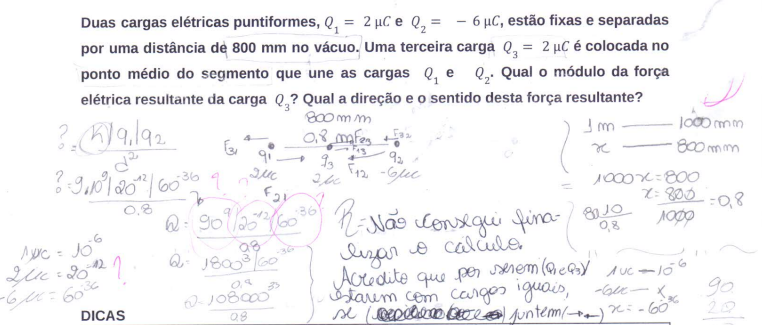
\includegraphics[width=1\textwidth]{fig/mtmasa3.png}
\label{fig:mtmasa3}
\caption*{Fonte: Extraído da produção dos Estudantes.}
\end{center}
\end{figure}

Com base na análise da ASA3, podemos concluir que a etapa que demandou mais auxílio (objetivo \ref{item:b}) foi a de Conteúdo, relacionada ao conhecimento específico da disciplina de Física. No entanto, ao longo do relato, tornou-se evidente que também foi necessário auxílio nas etapas de aplicação matemática. Apesar disso, os alunos não solicitaram esse auxílio por diversos motivos. Portanto, é importante considerar ambas as etapas como pontos de atenção para o desenvolvimento das habilidades dos alunos e garantir que eles se sintam encorajados a buscar ajuda quando necessário.

Com base nas informações do Professor e nos resultados dos alunos, constatamos que somente na última aplicação foi possível verificar uma evolução no processo de RP dos estudantes. No entanto, devido à dificuldade da turma em entender a proposta da ASA desde o início, não temos informações suficientes para responder ao objetivo \ref{item:c} sobre a evolução ao longo do tempo. Essa dificuldade pode ter influenciado os resultados e a compreensão do processo de RP, e destaca a importância de uma abordagem mais clara e direcionada em atividades futuras, para melhor acompanhamento do progresso dos alunos.

\begin{figure}[ht]
\begin{center}
\caption{Exemplo de dicas preferidas ao longo da ASA3.}
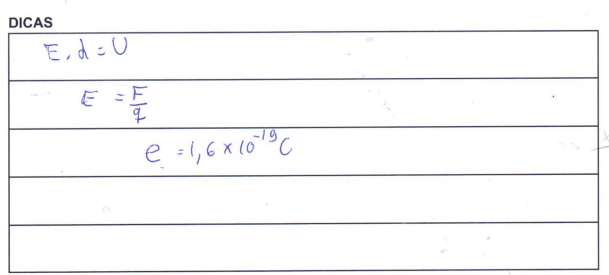
\includegraphics[width=1\textwidth]{fig/didasa3.png}
\label{fig:didiasa3}
\caption*{Fonte: Extraído da produção dos Estudantes.}
\end{center}
\end{figure}

É interessante notar que, de acordo com o relato do Professor, os alunos tinham uma preferência (objetivo \ref{item:d}) por dicas diretas, independentemente do tipo de dica oferecida - como mostrado na Figura \ref{fig:didiasa3}. Essa preferência pode estar relacionada à tentativa dos alunos de resolverem as questões com o mínimo de interferência externa possível. Além disso, eles pareciam estar buscando resolver as questões rapidamente, como se estivessem em uma situação de prova de vestibular, buscando otimizar o tempo disponível. Essa abordagem pode refletir a ansiedade e a pressão que os alunos podem sentir durante as avaliações importantes, como o vestibular, e evidencia a necessidade de equilibrar o uso das dicas com o desenvolvimento da autonomia e confiança dos estudantes em suas habilidades de RP.

\begin{table}[ht]
    \centering
    \caption{Respostas da ASA3 ao questionário final.}\label{tab:questASA3}
    \begin{tabular}{ccccc}
    \hline
       \textbf{Pergunta 1} & \textbf{Pergunta 2} & \textbf{Pergunta 3} & \textbf{Pergunta 4} & \textbf{Pergunta 5} \\ \hline
        1 & 1 & 1 & 4 & 5 \\ 
        3 & 1 & 4 & 1 & 1 \\ 
        4 & 3 & 5 & 2 & 2 \\ 
        5 & 1 & 3 & 3 & 5 \\ 
        3 & 3 & 4 & 2 & 3 \\ 
        5 & 5 & 5 & 3 & 5 \\ 
        3 & 3 & 4 & 4 & 4 \\ 
        5 & 5 & 5 & 4 & 2 \\ 
        3 & 3 & 5 & 1 & 5 \\ 
        5 & 4 & 5 & 3 & 4 \\ 
        5 & 4 & 5 & 4 & 3 \\ 
        5 & 4 & 4 & 3 & 4 \\ \hline
    \end{tabular}
    \caption*{Fonte: Construção do Autor.}
\end{table}

A Tabela \ref{tab:questASA3} apresenta as respostas dadas pelos alunos às perguntas do questionário, utilizando a escala Likert, ao término da aplicação da ASA3. O questionário completo está disponível no Apêndice \ref{ch:questASA}. Essas respostas fornecem informações importantes sobre a percepção dos alunos em relação ao processo de aplicações e suas experiências com a abordagem da ASA3.

Um primeiro fator relevante a ser observado é que 12 dos 14 alunos pesquisados responderam ao questionário, apesar de não ser obrigatório. Essa taxa de resposta corresponde a aproximadamente 86\% dos alunos pesquisados. Esse alto nível de participação indica que os alunos estavam interessados em compartilhar suas percepções e experiências sobre a ASA3, o que fortalece a validade das informações coletadas por meio do questionário.

Sobre o grau de dificuldade das questões (pergunta 1), em geral, a turma da ASA3 concordou que as questões apresentavam semelhança com as propostas em sala de aula. No entanto, os relatos deixados pelos alunos indicam que durante as aplicações eles enfrentavam maiores dificuldades do que costumavam ter ao resolver questões em sala de aula. Essa percepção pode ter contribuído para a redução no número de solicitações de dicas, já que alguns alunos sentiram-se mais desafiados e preferiram testar suas habilidades sem buscar auxílio imediato.

Os alunos se dividiram ao tentar avaliar se a ASA seria uma boa maneira de avaliá-los (pergunta 2). Pelos relatos obtidos, também no questionário (questão dissertativa), muitos alunos não gostam de resolver problemas e prefeririam ter seus conhecimentos avaliados de outras formas.

No entanto, é importante destacar que a RP é uma etapa importante e fundamental para o aprendizado da disciplina de Física, como já foi descrito nesta dissertação. Embora existam outros meios de avaliação, eles são complementares à RP e não podem ser substitutos completos dessa abordagem. Através da RP, os alunos desenvolvem habilidades de raciocínio, pensamento crítico e aplicação prática do conhecimento adquirido em diferentes situações.

Portanto, a ASA se apresenta como uma ferramenta valiosa para auxiliar os estudantes na melhoria de suas competências em RP, e, ao longo do processo, pode contribuir para que eles se sintam mais confiantes e preparados para enfrentar os desafios acadêmicos, incluindo as avaliações de vestibulares e ENEM, que também valorizam a habilidade de resolver problemas de forma eficaz.

Quando perguntados sobre a eficácia das dicas fornecidas durante a RP (pergunta 3), a maioria dos alunos concordou que elas foram úteis. Isso indica que os alunos sentiram que houve uma melhora em seus resultados após fazerem uso das dicas durante o processo de resolução das questões. Essa percepção reforça o papel positivo das dicas na compreensão dos conteúdos e na superação das dificuldades encontradas durante as aplicações da ASA3.

Ao serem questionados sobre o autoconhecimento de suas habilidades e desempenho ao longo das aplicações (pergunta 4), a turma apresentou uma divisão de opiniões, mas com uma leve tendência a concordar que entenderam melhor suas competências e dificuldades. Essa percepção é um fator relevante, pois demonstra que os alunos estão, em parte, se tornando mais conscientes de suas habilidades e áreas em que precisam melhorar. Esse autoconhecimento pode ser um ponto positivo para o aprimoramento do aprendizado, uma vez que permite que eles identifiquem suas forças e fraquezas e busquem formas de aperfeiçoar suas habilidades.


De acordo com as respostas dos alunos à pergunta sobre a possibilidade de haver mais aplicações ao longo do trimestre, a turma, em geral, concordou com essa ideia. Isso indica que a maioria dos estudantes gostaria de repetir esse processo mais vezes. 

Essa aceitação pode estar conectada ao fato de que os alunos levaram um tempo para compreender como o processo da ASA pode auxiliá-los em seu aprendizado. Com o passar do tempo e a experiência com as aplicações, eles perceberam os benefícios desse método e, consequentemente, demonstraram interesse em tê-lo mais vezes no decorrer do trimestre para aprimorar suas habilidades e superar dificuldades.

Com base na análise do questionário, é possível afirmar que o interesse na RP não apenas se manteve ao longo do trimestre (objetivo \ref{item:e}), mas também aumentou. Essa constatação pode ser atribuída às boas experiências que os alunos tiveram ao participar das aplicações da ASA e após compreenderem a forma de funcionamento desse método de aprendizagem. A medida em que os alunos se familiarizaram com o processo e perceberam os benefícios das aplicações, o interesse e a motivação para se engajar no processo de RP foram fortalecidos, demonstrando um crescente engajamento com o método ao longo do trimestre.
